%%
% Modificación de una plantilla de Latex para adaptarla al castellano.
%%

%%%%%%%%%%%%%%%%%%%%%
% Thin Sectioned Essay
% LaTeX Template
% Version 1.0 (3/8/13)
%
% This template has been downloaded from:
% http://www.LaTeXTemplates.com
%
% Original Author:
% Nicolas Diaz (nsdiaz@uc.cl) with extensive modifications by:
% Vel (vel@latextemplates.com)
%
% License:
% CC BY-NC-SA 3.0 (http://creativecommons.org/licenses/by-nc-sa/3.0/)
%
%%%%%%%%%%%%%%%%%%%%%

%----------------------------------------------------------------------------------------
%	PACKAGES AND OTHER DOCUMENT CONFIGURATIONS
%----------------------------------------------------------------------------------------

\documentclass[a4paper, 11pt]{article} % Font size (can be 10pt, 11pt or 12pt) and paper size (remove a4paper for US letter paper)

\usepackage[protrusion=true,expansion=true]{microtype} % Better typography
\usepackage{graphicx} % Required for including pictures
\usepackage[usenames,dvipsnames]{color} % Coloring code
\usepackage{wrapfig} % Allows in-line images
\usepackage[utf8]{inputenc}
\usepackage{enumerate}
\usepackage{enumitem}

% Imágenes
\usepackage{graphicx} 

\usepackage{amsmath}
% para importar svg
%\usepackage[generate=all]{svgfig}

% sudo apt-get install texlive-lang-spanish
\usepackage[spanish]{babel} % English language/hyphenation
\selectlanguage{spanish}
% Hay que pelearse con babel-spanish para el alineamiento del punto decimal
\decimalpoint
\usepackage{dcolumn}
\newcolumntype{d}[1]{D{.}{\esperiod}{#1}}
\makeatletter
\addto\shorthandsspanish{\let\esperiod\es@period@code}
\makeatother

\usepackage{longtable}
\usepackage{tabu}
\usepackage{supertabular}

\usepackage{multicol}
\newsavebox\ltmcbox

% Para algoritmos
\usepackage{algorithm}
\usepackage{algorithmic}
\usepackage{amsthm}

% Para matrices
\usepackage{amsmath}

% Símbolos matemáticos
\usepackage{amssymb}
\usepackage{accents}
\let\oldemptyset\emptyset
\let\emptyset\varnothing

\usepackage[hidelinks]{hyperref}

\usepackage[section]{placeins} % Para gráficas en su sección.
\usepackage[T1]{fontenc} % Required for accented characters
\newenvironment{allintypewriter}{\ttfamily}{\par}
\setlength{\parindent}{0pt}
\parskip=8pt
\linespread{1.05} % Change line spacing here, Palatino benefits from a slight increase by default

\makeatletter
\renewcommand\@biblabel[1]{\textbf{#1.}} % Change the square brackets for each bibliography item from '[1]' to '1.'
\renewcommand{\@listI}{\itemsep=0pt} % Reduce the space between items in the itemize and enumerate environments and the bibliography
\newcommand{\imagen}[2]{\begin{center} \includegraphics[width=90mm]{#1} \\#2 \end{center}}
\newcommand{\RFC}[1]{\href{https://www.ietf.org/rfc/rfc#1.txt}{RFC-#1}}

\renewcommand{\maketitle}{ % Customize the title - do not edit title and author name here, see the TITLE block below
\begin{center} % Center align
{\Huge\@title} % Increase the font size of the title
\end{center}

\vspace{20pt} % Some vertical space between the title and author name

\begin{flushright} % Right align
{\large\@author} % Author name
\\\@date % Date

\vspace{40pt} % Some vertical space between the author block and abstract
\end{flushright}
}
%----------------------------------------------------------------------------------------
%	TITLE
%----------------------------------------------------------------------------------------

\title{\textbf{Monitorización de Servicios}\\ % Title
\vspace{20 pt}
Ingeniería de Servidores \\Memoria de la Práctica 3} % Subtitle

\author{\textsc{Adrián Portillo Sánchez} % Author
\\{\textit{Universidad de Granada}}} % Institution

\date{\today} % Date

%----------------------------------------------------------------------------------------
\setcounter{secnumdepth}{0}

\begin{document}
\maketitle
\pagebreak
\tableofcontents
\pagebreak
\listoffigures
\pagebreak


\section{Cuestión 1}
\textbf{a) ¿Qué archivo le permite ver qué programas se han instalado con el gestor de paquetes?\\ b) ¿Qué significan las terminaciones .1.gz o .2.gz de los archivos en ese directorio?}\\ 

\begin{itemize}
\item[a)]\cite{1}\cite{2}En el caso de centOS el archivo que guarda los paquetes que han sido instalados en el sistema se encuentra en \textit{/var/log} y se llama \textit{yum.log}, este archivo contiene los paquetes que han sido instalados y eliminados con la herramienta yum. En el caso de Ubuntu este registro se encuentra en el mismo directorio con el nombre \textit{dpkg.log} y también muestra los paquetes instalados y borrados del sistema. El formato de ambos archivos es:
\begin{verbatim}
[fecha] [Installed/Deleted/Updated]:    [paquete] #CentOS
[fecha] [Accion]                        [paquete] #Ubuntu
\end{verbatim}

\begin{figure}[H]
\centering 
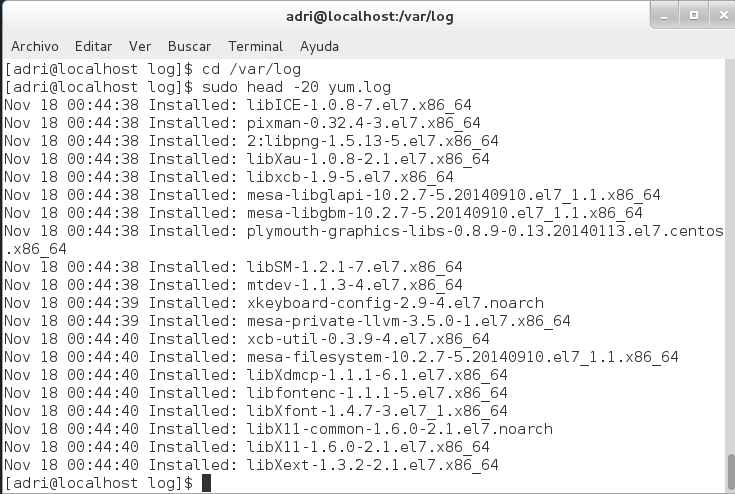
\includegraphics[width=1\linewidth]{paquetes1.png} 
\caption{Archivo /var/log/yum.log en CentOS.} 
\label{contexto:figura} 
\end{figure}

\begin{figure}[H]
\centering 
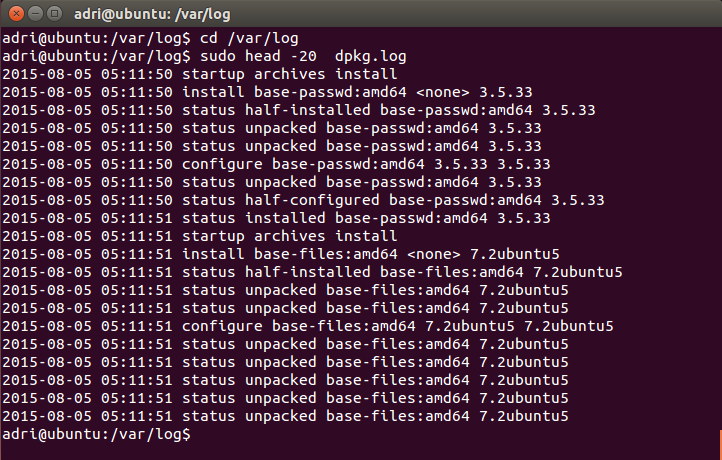
\includegraphics[width=1\linewidth]{paquetes2.png} 
\caption{Archivo /var/log/dpkg.log en Ubuntu.} 
\label{contexto:figura} 
\end{figure}


\item[b)] \cite{3} \cite{4} Son archivos de registro que han sido comprimidos según las especificaciones de generación del propio archivo de registro, normalmente el tamaño que se ha definido para que ocupen. Estos archivos se generan por un proceso de rotación del sistema, que normalmente es \textit{logrotate}, que se encuentra en \textit{/etc/cron.daily} y es un script con una tarea que se ejecuta diariamente, se encargará de dar una rotación de manera automática que comprime, y borra los registros de manera diaria, semanal, mensual... Dependiendo de la configuración que se posea, ya que esta se puede modificar en el archivo \textit{/etc/logrotate.conf}. Por lo que esos archivos son versiones más antiguas del registro, comprimidas y con el número del archivo con el formato <numero>.gz, que es el número de generación de archivo (cuanto mayor sea el número más antiguo será el log).
\end{itemize}

\pagebreak

\section{Cuestión Opcional 1}
\textbf{Indique los pasos que ha seguido, comandos empleados y significado de los mismos. Junto a cada comando, presente las líneas del registro del RAID que son significativas en cada paso: indicación de fallo, reemplazo, inicio y finalización de la reconstrucción del RAID.}\\

\cite{5} En primer lugar se ha utilizado la máquina virtual de Ubuntu server de la práctica 1 y se ha usado como ayuda la referencia \cite{6} \cite{7} para finalizar la cuestion. Debido a que no tiene interfaz gráfica me ha sido más cómodo usar directamente el comando \textit{cat} que monitorizarlo pero el resultado seria el mostrado. Primero revisamos el estado del registro (figura 3):
\begin{figure}[H]
\centering 
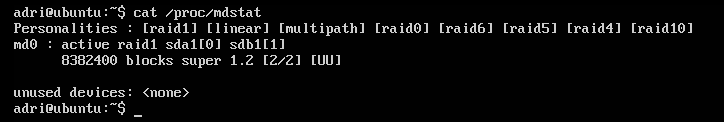
\includegraphics[width=1\linewidth]{mdadm1.png} 
\caption{Registro con todo los discos correctos.} 
\label{contexto:figura} 
\end{figure}
Ahora vamos a producir un error en el disco con el comando \textit{''mdadm --manage /dev/md0 --fail /dev/sdb1''}, este comando nos permite administrar dispositivos que conformen un RAID, en especifico el comando con la opción \textit{--manage} nos permite añadir, quitar o incluso producir un fallo en el disco con la opción \textit{--fail} (figura 4):
\begin{figure}[H]
\centering 
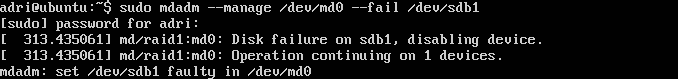
\includegraphics[width=1\linewidth]{mdadm2.png} 
\caption{Producción de fallo al disco /dev/sdb1.} 
\label{contexto:figura} 
\end{figure}

\pagebreak

Volvemos a comprobar el registro y damos cuenta de que el disco sdb1 está marcado con una \textit{(F)} que indica se ha producido un fallo en él. Otra diferencia es \textit{[2/1][U\_]} anteriormente se marcaba como \textit{[2/2][UU]} esto es muestra de que uno de los discos esta ''degradado'' (figura 5):
\begin{figure}[H]
\centering 
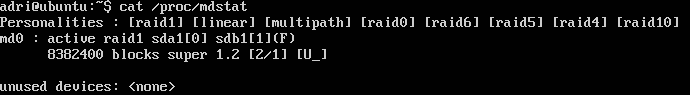
\includegraphics[width=1\linewidth]{mdadm3.png} 
\caption{Registro indicando el fallo de sdb1.} 
\label{contexto:figura} 
\end{figure}
Para quitar el disco que ha fallado del sistema hacemos uso del comando \textit{''mdadm --manage /dev/md0 --remove /dev/sdb1''} que nos permite exactamente eso, deshabilitar el disco (figura 6) y volvemos a comprobar el registro (figura 7):
\begin{figure}[H]
\centering 
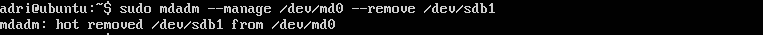
\includegraphics[width=1\linewidth]{mdadm4.png} 
\caption{Quitando el disco del sistema.} 
\label{contexto:figura} 
\end{figure}
\begin{figure}[H]
\centering 
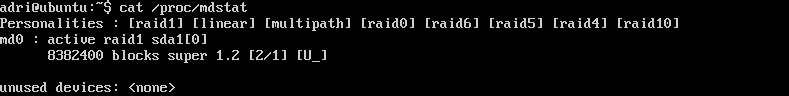
\includegraphics[width=1\linewidth]{mdadm5.png} 
\caption{Registro sin el disco sdb1.} 
\label{contexto:figura} 
\end{figure}

En este momento es cuando se tiene que reponer el disco por otro que este vacio, en un sistema real se tendria que sustituir el disco por otro y automáticamente se iniciaria el proceso de recuperación en nuestro caso añadimos un disco al sistema del mismo tamaño con el comando \textit{''mdadm --manage /dev/md0 --add /dev/sdb1''} y verificamos que se produce la recuperación (figuras 8-9):
\begin{figure}[H]
\centering 
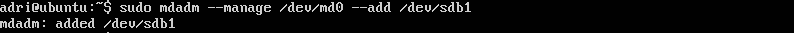
\includegraphics[width=1\linewidth]{mdadm6.png} 
\caption{Reposición del disco.} 
\label{contexto:figura} 
\end{figure}
\begin{figure}[H]
\centering 
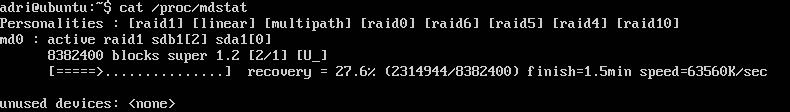
\includegraphics[width=1\linewidth]{mdadm7.png} 
\caption{Registro mostrando la recuperación del disco.} 
\label{contexto:figura} 
\end{figure}
Por último se muestra el estado final del \textit{RAID} ya con el disco sustituido y recuperado como podemos apreciar ahora \textit{[2/2][UU]}, es decir no hay error en los discos están los dos operativos y parece que \textit{sdb1[2]} se indica con un 2 por que se ha producido una sustitución de disco (figura 10):
\begin{figure}[H]
\centering 
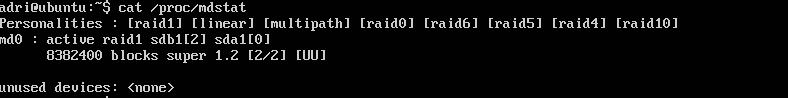
\includegraphics[width=1\linewidth]{mdadm8.png} 
\caption{Estado final de los discos de sistema.} 
\label{contexto:figura} 
\end{figure}

\section{Cuestión 2}
\textbf{¿qué archivo ha de modificar para programar una tarea? Escriba la línea necesaria para ejecutar una vez al día una copia del directorio \~/codigo a \~/seguridad/\$fecha donde \$fecha es la fecha actual (puede usar el comando date).}\\

\cite{8} Para programar una tarea se ha de modificar el archivo \textit{/etc/crontab} o el archivo \textit{/var/spool/cron}, también se puede editar con la orden \textit{crontab -e}.\\
Para crear las copias diarias creamos un script llamado \textit{copia\_diaria.sh} con el siguiente contenido:
\begin{verbatim}
#!/bin/bash
fecha=`date +"%m-%d-%y"`
directorio_origen=~/codigo/*
directorio_final=~/seguridad/$fecha
mkdir $directorio_final
cp $directorio_origen $directorio_final
\end{verbatim}
El script obtiene la fecha del dia con el comando date y copia el contenido del directorio \textit{\~/codigo} y lo pega en el directorio \textit{\~/seguridad/\$fecha}, es decir crea un directorio con la fecha actual y pega los archivos en dicha carpeta. \\
Ahora vamos a editar el archivo \textit{/etc/crontab} para que este script se ejecute diariamente:
\begin{verbatim}
SHELL=/bin/bash
PATH=/sbin:/bin:/usr/sbin:/usr/bin
MAILTO=root

# For details see man 4 crontabs

# Example of job definition:
# .---------------- minute (0 - 59)
# |  .------------- hour (0 - 23)
# |  |  .---------- day of month (1 - 31)
# |  |  |  .------- month (1 - 12) OR jan,feb,mar,apr ...
# |  |  |  |  .---- day of week (0 - 6) (Sunday=0 or 7) OR sun,mon,tue,wed,thu,fri,sat
# |  |  |  |  |
# *  *  *  *  * user-name  command to be executed

00 00 * * * /home/adri/copia_diaria.sh
\end{verbatim}
Esto quiere decir que \textit{copia\_diaria.sh} se ejecutará a las 00:00 cada día de la semana.

\section{Cuestión 3}
\textbf{Pruebe a ejecutar el comando, conectar un dispositivo USB y vuelva a ejecutar el comando. Copie y pegue la salida del comando. (considere usar dmesg | tail). Comente qué observa en la información mostrada.}\\

\cite{9} Las salidas que hacen mención a la conexión del dispositivo USB son las siguientes:
\begin{verbatim}
adri@ubuntu:~\$ dmesg | tail -25
...
[ 3859.155240] usb 1-1: new full-speed USB device number 2
using ohci-pci
[ 3859.342210] usb 1-1: New USB device found, idVendor=058f,
idProduct=6387 
[ 3859.342217] usb 1-1: New USB device strings: Mfr=1, Product=2,
SerialNumber=3 
[ 3859.342221] usb 1-1: Product: Mass Storage 
[ 3859.342225] usb 1-1: Manufacturer: Generic 
[ 3859.342228] usb 1-1: SerialNumber: 3DC5D1E7 
[ 3859.675775] usb-storage 1-1:1.0: USB Mass Storage device detected 
[ 3859.679591] scsi3 : usb-storage 1-1:1.0 
[ 3859.679675] usbcore: registered new interface driver usb-storage 
[ 3860.717934] scsi 3:0:0:0: Direct-Access Generic Flash Disk
8.07 PQ: 0 ANSI: 4 
[ 3860.724190] sd 3:0:0:0: Attached scsi generic sg2 type 0 
[ 3860.768601] sd 3:0:0:0: [sdb] 15974400 512-byte
logical blocks: (8.17 GB/7.61 GiB) 
[ 3860.780251] sd 3:0:0:0: [sdb] Write Protect is off 
[ 3860.780257] sd 3:0:0:0: [sdb] Mode Sense: 23 00 00 00 
[ 3860.790310] sd 3:0:0:0: [sdb] Write cache: disabled, 
read cache: enabled, doesn't support DPO or FUA 
[ 3860.873104] sdb: sdb1 
[ 3860.962896] sd 3:0:0:0: [sdb] Attached SCSI removable disk 
[ 3863.743125] FAT-fs (sdb1): Volume was not properly unmounted.
Some data may be corrupt. Please run fsck. 
[ 3863.743222] SELinux: initialized (dev sdb1, type vfat), uses
genfs_contexts 
[ 3917.288285] hrtimer: interrupt took 811643 ns
\end{verbatim}

Aquí podemos observar los mensajes del sistema cuando el dispositivo usb se conectó, en primer lugar el sistema lista los datos del dispositivo (datos generales, id del vendedor y del producto, nombre del producto fabricante y número de serie); tras esto se pueden observar mensajes de la detección del dispositivo y sus drivers asociados, así como distintas configuraciones sobre el trato al dispositivo (protección de escritura, cachés...). Por último, se le da un identificador de disco para el sistema.\\
En las últimas líneas vemos que el dispositivo se desconectó de forma incorrecta, y el tiempo que tomó la interrupción causada.\\
Aquí tenemos otro ejemplo conectando un ratón usb.

\begin{figure}[H]
\centering 
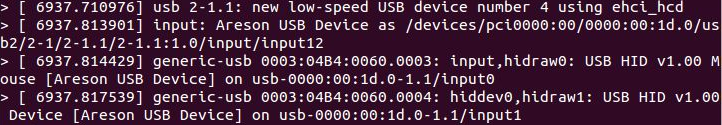
\includegraphics[width=0.8\linewidth]{usb.png} 
\caption{Ejemplo conectando un ratón.} 
\label{contexto:figura} 
\end{figure}

\pagebreak

\section{Cuestión 4}
\textbf{Ejecute el monitor de ''System Performance'' y muestre el resultado. Incluya capturas de pantalla y comente la información que aparece.}\\

\cite{10}Para ejecutar el monitor de rendimiento hemos utilizado el comando \textit{perfmon} en la consola de windows, como podemos observar tenemos un resumen del sistema que presenta información general del mismo (figura 12):

\begin{itemize}
\item \textbf{Información del disco físico:} Porcentaje de tiempo inactivo y longitud de cola, para cada disco C,E,E en este caso puesto que se tiene en el sistema un disco reflejado, se muestran los datos anteriores de cada uno de ellos y un a columna total que realiza la media.
\item \textbf{Información del procesador:} Muestra el porcentaje de tiempo de interrupción y de procesador además del estado de detención de todos los procesadores del sistema y un total que realiza la media de todos.
\item \textbf{Información del interfaz de red:} Muestra el total de bytes de cada adaptador web en el sistema.
\item \textbf{Información de la memoria:} Informa de los errores de cache, la memoria libre en ese momento y el porcentaje de bytes en uso.
\end{itemize}

Además por defecto tenemos el monitor de rendimiento que nos informa del porcentaje de procesador (figura 13), además se nos da la posibilidad de crear nuestros propios recopiladores de datos que pueden realizar una serie de informes con los datos que se especifican a la hora de configuración (figura 13).
\begin{figure}[H]
\centering 
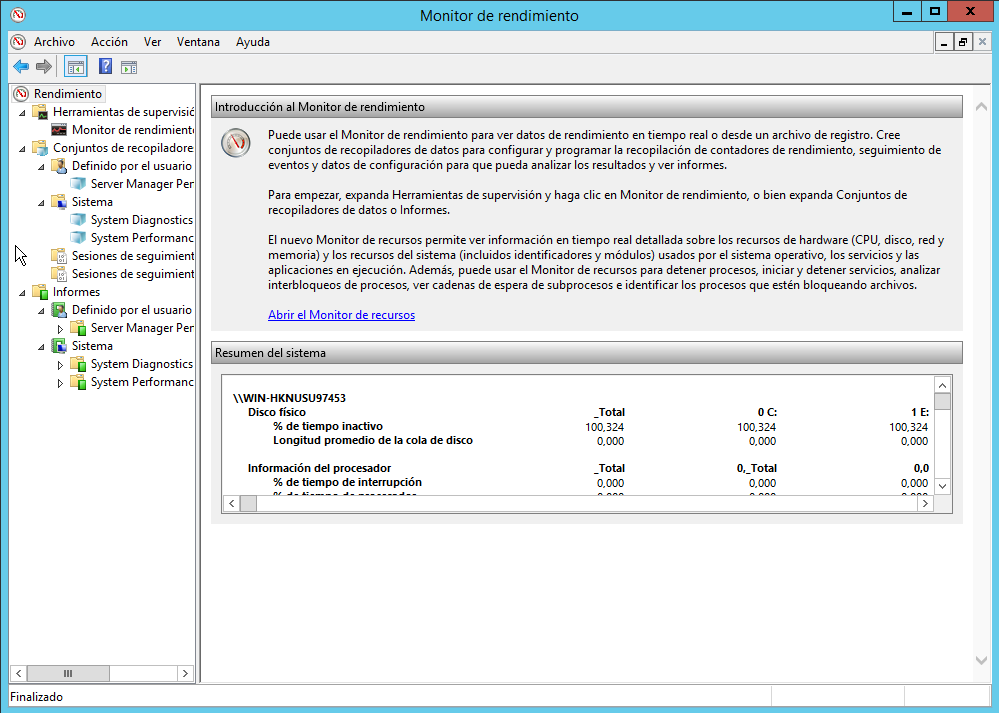
\includegraphics[width=0.8\linewidth]{perfmon1.png} 
\caption{Pantalla de inicio Perfmon.} 
\label{contexto:figura} 
\end{figure}
\begin{figure}[H]
\centering 
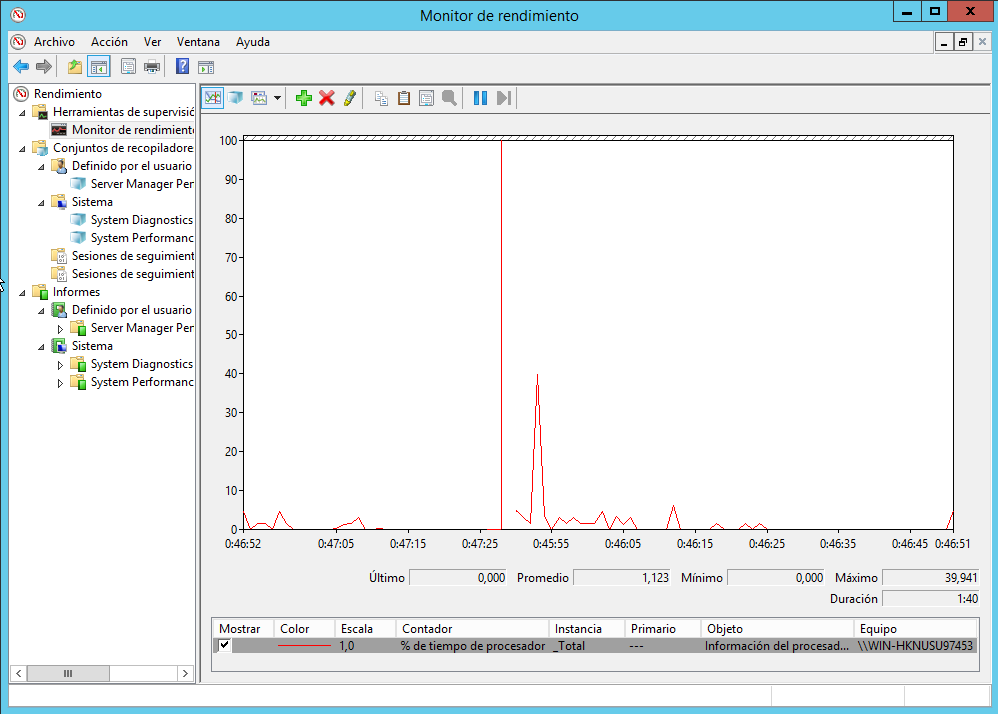
\includegraphics[width=0.8\linewidth]{perfmon2.png} 
\caption{Monitor de rendimiento Perfmon.} 
\label{contexto:figura} 
\end{figure}

\pagebreak

\section{Cuestión 5}
\textbf{Cree un recopilador de datos definido por el usuario (modo avanzado) que incluya tanto el contador de rendimiento como los datos de seguimiento:
\begin{itemize}
\item [] Todos los referentes al procesador, al proceso y al servicio web.
\item [] Intervalo de muestra 15 segundos
\item [] Almacene el resultado en el directorio Escritorio/logs
\end{itemize}
Incluya las capturas de pantalla de cada paso.}\\

\cite{11} Para crear un nuevo conjunto de recopiladores de datos nos dirigimos a los recopiladores definidos por el usuario y seleccionamos la opción Nuevo, obtendremos una ventana (figura 14) en la que podremos poner nombre a nuestro conjunto de recopiladores, seleccionamos crear manualmente y se selecciona contador de rendimiento y datos de seguimiento de eventos (figura 15). Ahora tenemos que seleccionar todos los datos referentes a el procesador, proceso y servidor web para ello los seleccionamos con todas las instancias del objeto (en mi caso el resultado de elegir \_total y <Todas las instancias> fue el mismo)(figura 16), por último confirmamos los contadores de rendimiento (figura 17). Por último seleccionamos el la carpeta que guardará los datos y establecemos la carpeta Escritorio/log y finalizamos la creación (figura 18), para que se inicie el recopilador tenemos que iniciarlo en el monitor de rendimiento y se crearian los informes (figura 19) con la información que se pide monitorizar cada 15 segundos (figura 20).

\begin{figure}[H]
\centering 
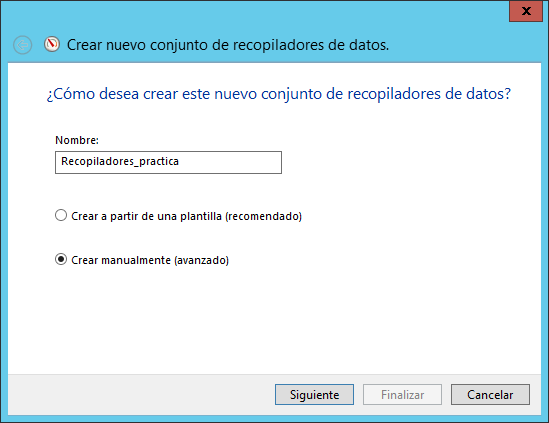
\includegraphics[width=0.8\linewidth]{perfmon3.png} 
\caption{Creación nuevo conjunto de recopiladores.} 
\label{contexto:figura} 
\end{figure}
\begin{figure}[H]
\centering 
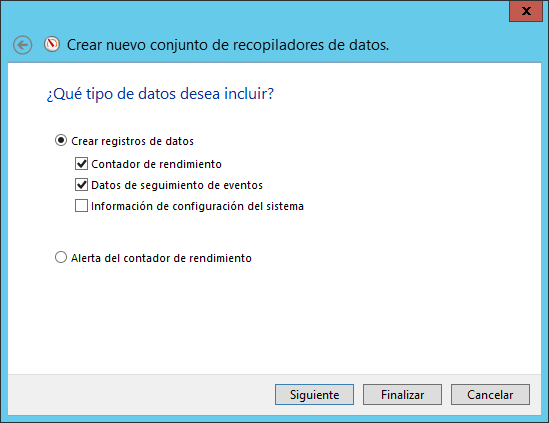
\includegraphics[width=0.8\linewidth]{perfmon4.png} 
\caption{Añadiendo registros de contador de rendimiento y datos de seguimiento de eventos.} 
\label{contexto:figura} 
\end{figure}
\begin{figure}[H]
\centering 
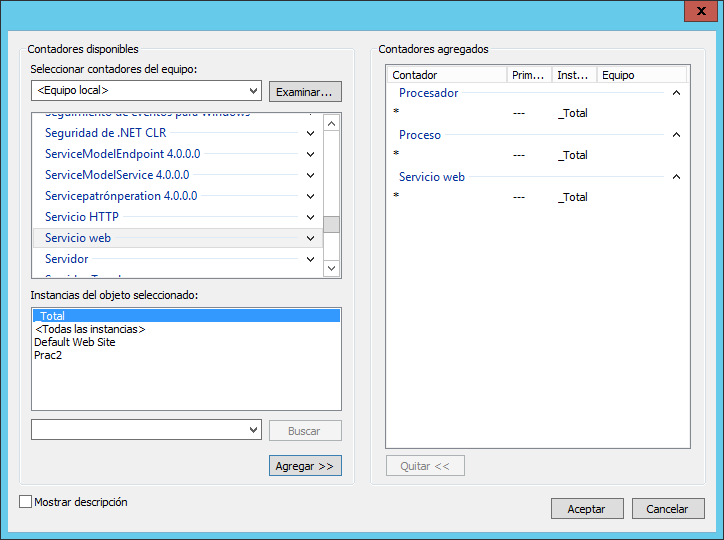
\includegraphics[width=0.8\linewidth]{perfmon5.png} 
\caption{Añadiendo contadores: Procesador, proceso, servicio web.} 
\label{contexto:figura} 
\end{figure}
\begin{figure}[H]
\centering 
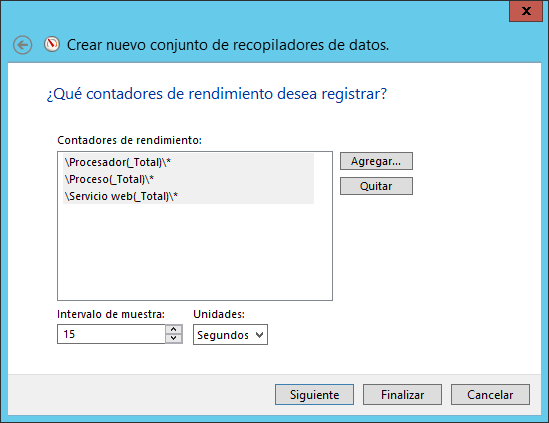
\includegraphics[width=0.8\linewidth]{perfmon6.png} 
\caption{Estableciendo intervalo de muestra.} 
\label{contexto:figura} 
\end{figure}
\begin{figure}[H]
\centering 
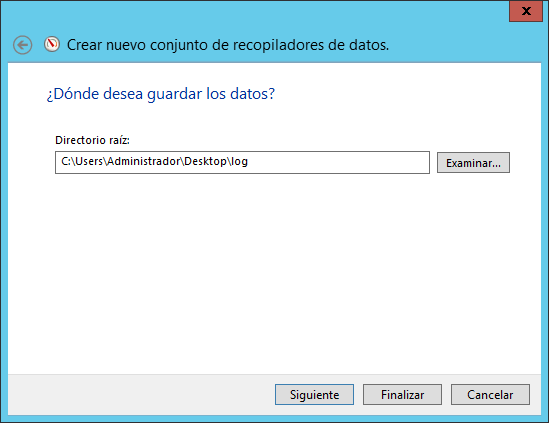
\includegraphics[width=0.8\linewidth]{perfmon7.png} 
\caption{Estableciendo carpeta log.} 
\label{contexto:figura} 
\end{figure}
\begin{figure}[H]
\centering 
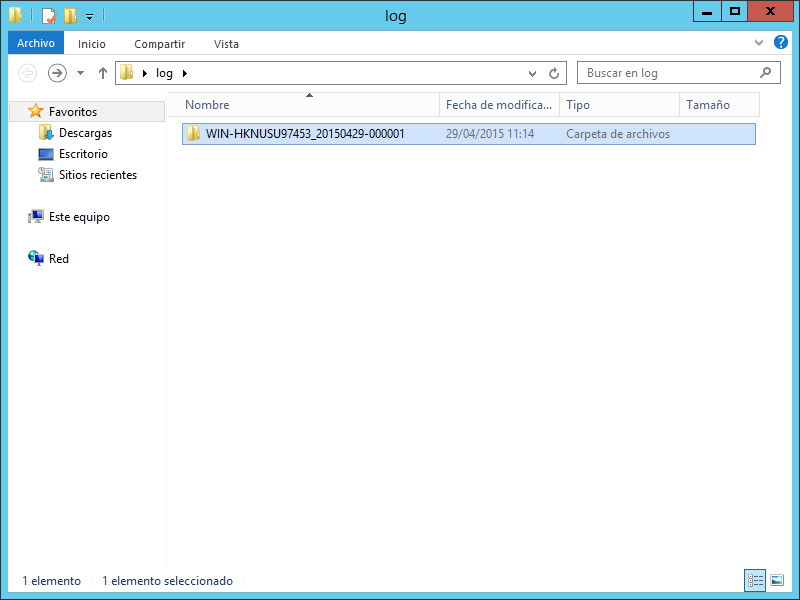
\includegraphics[width=0.8\linewidth]{perfmon8.png} 
\caption{Carpeta log.} 
\label{contexto:figura} 
\end{figure}
\begin{figure}[H]
\centering 
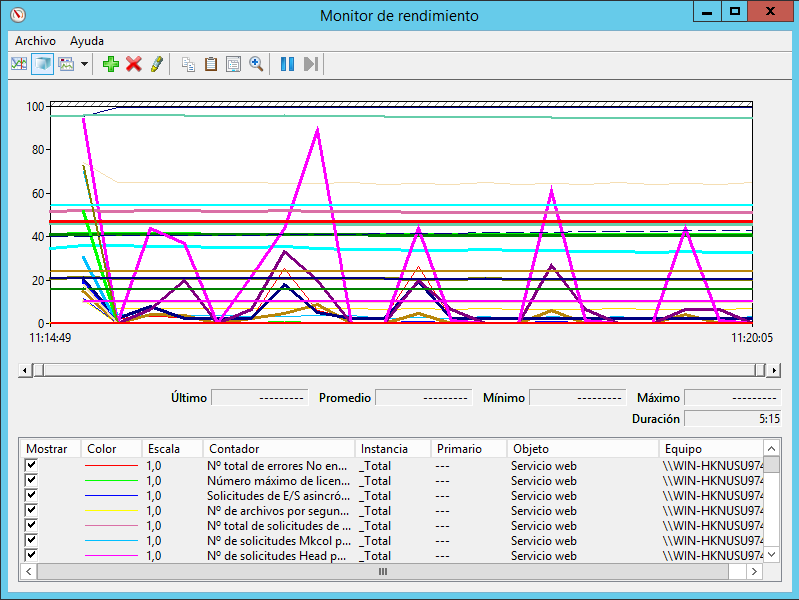
\includegraphics[width=0.8\linewidth]{perfmon9.png} 
\caption{Monitor de rendimiento con los datos cada 15 segundos.} 
\label{contexto:figura} 
\end{figure}

\pagebreak

\section{Cuestión 6}
\textbf{Instale alguno de los monitores comentados arriba en su máquina y pruebe a ejecutarlos (tenga en cuenta que si lo hace en la máquina virtual, los resultados pueden no ser realistas). Alternativamente, busque otros monitores para hardware comerciales o de código abierto para Windows y Linux.}\\

\cite{12}He decidido instalar paso a paso lm-sensors y su GUI xsensors en Ubuntu Server, a continuación mostraré diversas capturas de pantalla con los pasos realizados, y los resultados obtenidos:
\begin{figure}[H]
\centering 
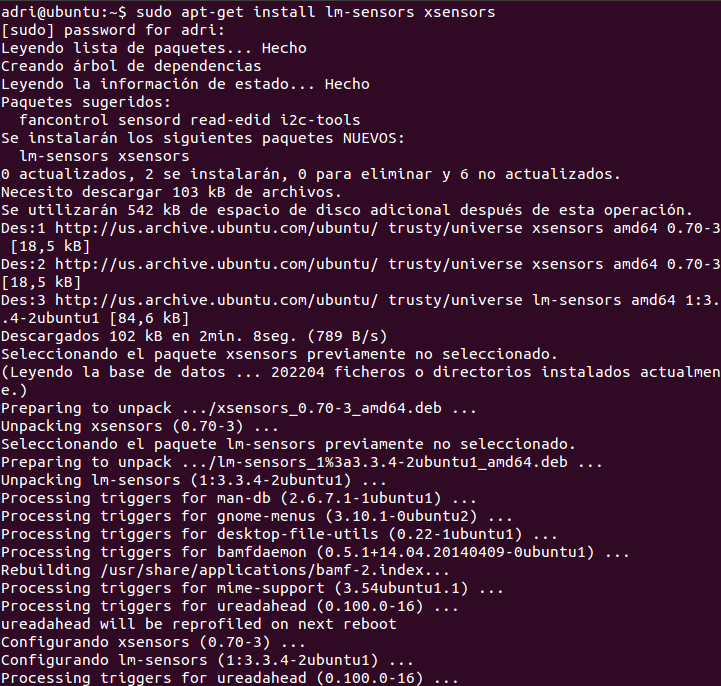
\includegraphics[width=0.8\linewidth]{lmsensors1.png} 
\caption{Instalando lm-sensors y su GUI xsensors.} 
\label{contexto:figura} 
\end{figure}

\pagebreak

Usamos sensors-detect para conocer que sensores se encuentran disponibles en nuestro sistema, para ello responderemos afirmativamente a todas las pruebas que solicite hacer el programa.
\begin{figure}[H]
\centering 
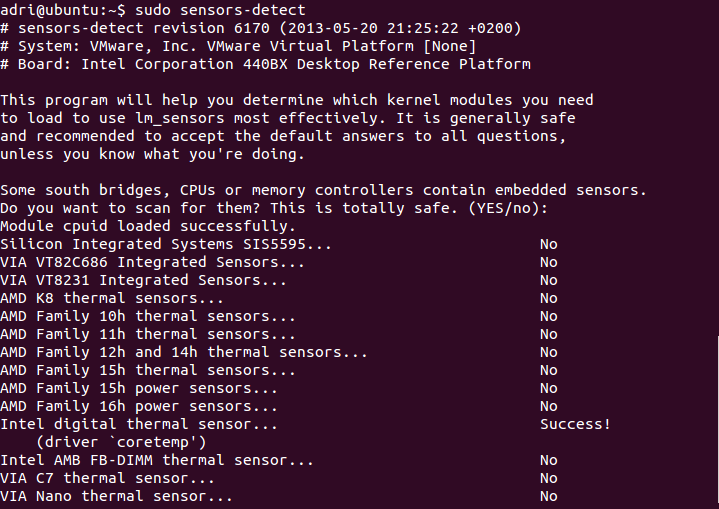
\includegraphics[width=0.8\linewidth]{lmsensors2.png} 
\caption{Detección de sensores y configuración inicial.} 
\label{contexto:figura} 
\end{figure}

Una vez finalizadas las pruebas, el programa nos indicará los módulos que debemos añadir a nuestra configuración para que se puedan hacer las monitorizaciones disponibles, además de darnos la opción de añadirlos directamente a nuestra configuración.
\begin{figure}[H]
\centering 
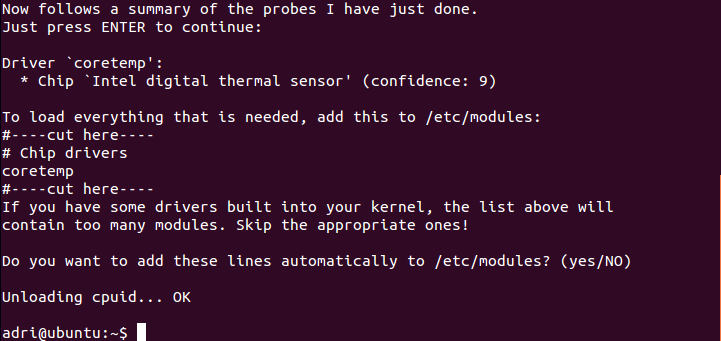
\includegraphics[width=0.8\linewidth]{lmsensors3.png} 
\caption{Módulos añadidos a configuración, se hace automáticamente.} 
\label{contexto:figura} 
\end{figure}

\pagebreak

Ahora ya podremos obtener las mediciones en entorno texto o gráfico según como llamemos al programa. Para el modo texto usamos “sensors”:
\begin{figure}[H]
\centering 
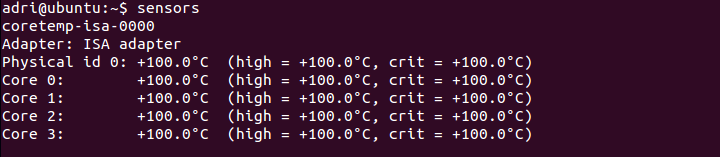
\includegraphics[width=0.8\linewidth]{lmsensors4.png} 
\caption{Ejecución de lm-sensors en línea de comandos.} 
\label{contexto:figura} 
\end{figure}

Para el modo gráfico usamos “xsensors”:
\begin{figure}[H]
\centering 
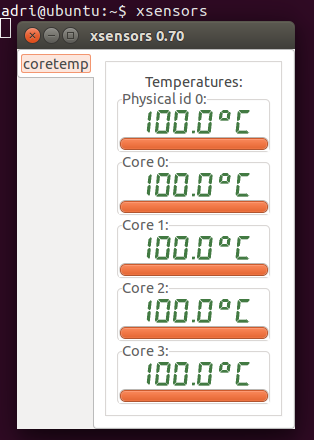
\includegraphics[width=0.4\linewidth]{lmsensors5.png} 
\caption{Ejecución de xsensors, la interfaz gráfica de lm-sensors.} 
\label{contexto:figura} 
\end{figure}

Al haberse ejecutado las pruebas en una máquina virtual, las pruebas no son realistas de hecho la temperatura de mi CPU no llega ni a un tercio de la marcada por xsensors:
\begin{figure}[H]
\centering 
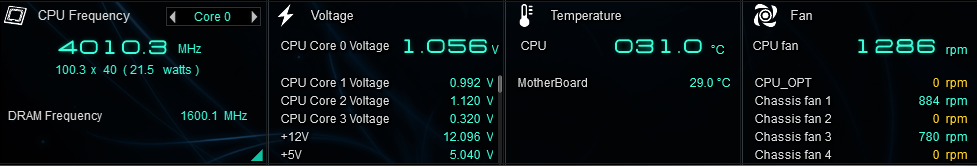
\includegraphics[width=1\linewidth]{lmsensors6.png} 
\caption{Mediciones reales de mi CPU.} 
\label{contexto:figura} 
\end{figure}

\pagebreak

\section{Cuestión 7}
\textbf{Visite la web del proyecto y acceda a la demo que proporcionan (\url{http://demo.munin-monitoring.org/}) donde se muestra cómo monitorizan un servidor. Monitorice varios parámetros y haga capturas de pantalla de lo que está mostrando comentando qué observa.}\\

\cite{13}A continuación mostraré algunos de los parámetros monitorizados en diversas capturas de pantalla:

\begin{figure}[H]
\centering 
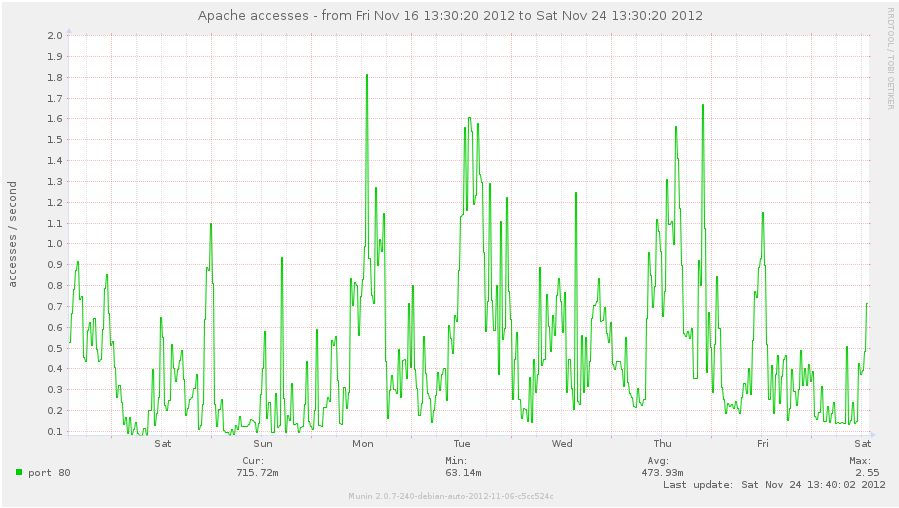
\includegraphics[width=0.8\linewidth]{munin1.png} 
\caption{Accesos al servidor Apache durante la última semana.} 
\label{contexto:figura} 
\end{figure}
\begin{figure}[H]
\centering 
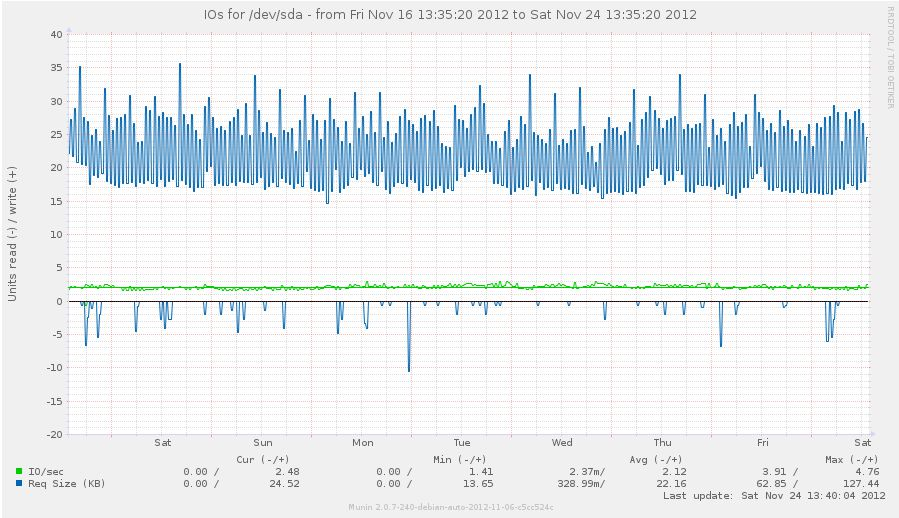
\includegraphics[width=0.8\linewidth]{munin2.png} 
\caption{Operaciones de E/S en la unidad de disco duro durante la última semana.} 
\label{contexto:figura} 
\end{figure}
\begin{figure}[H]
\centering 
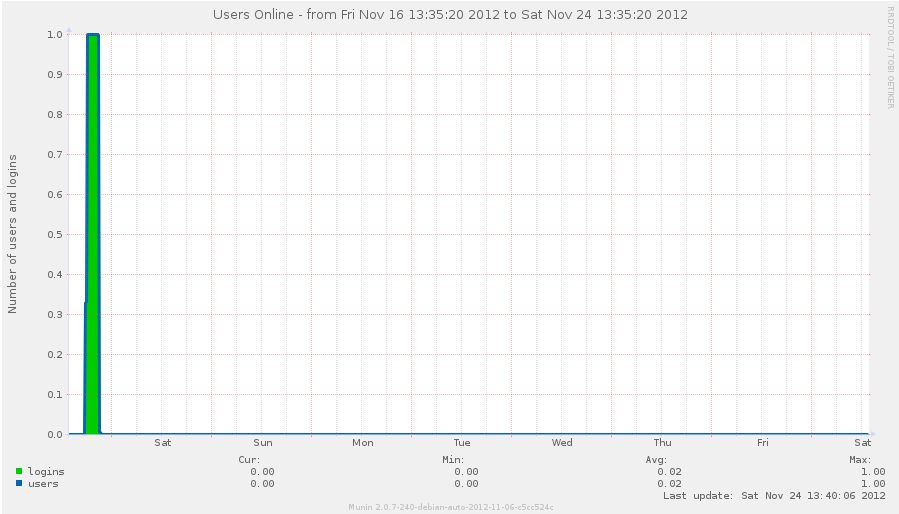
\includegraphics[width=0.8\linewidth]{munin3.png} 
\caption{Usuarios conectados durante la última semana.} 
\label{contexto:figura} 
\end{figure}
\begin{figure}[H]
\centering 
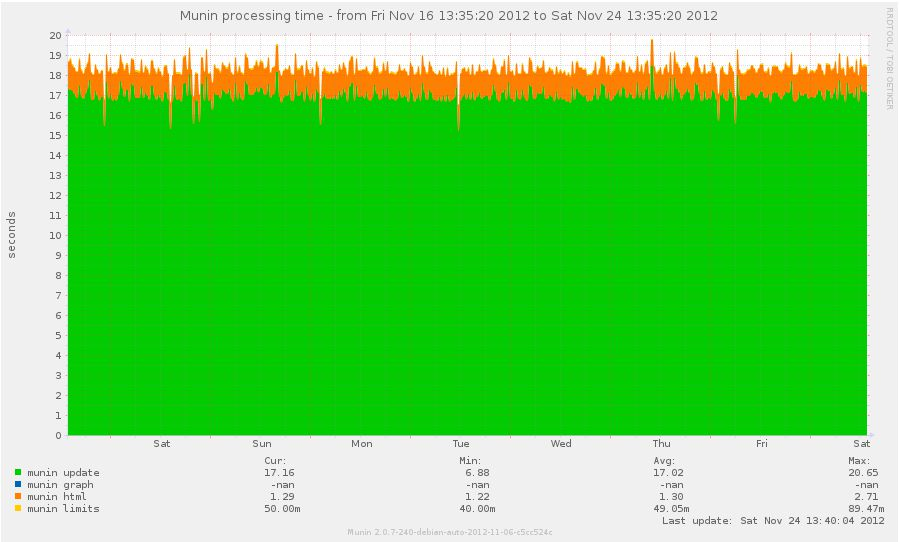
\includegraphics[width=0.8\linewidth]{munin4.png} 
\caption{Tiempo de procesamiento de Munin durante la última semana.} 
\label{contexto:figura} 
\end{figure}
\begin{figure}[H]
\centering 
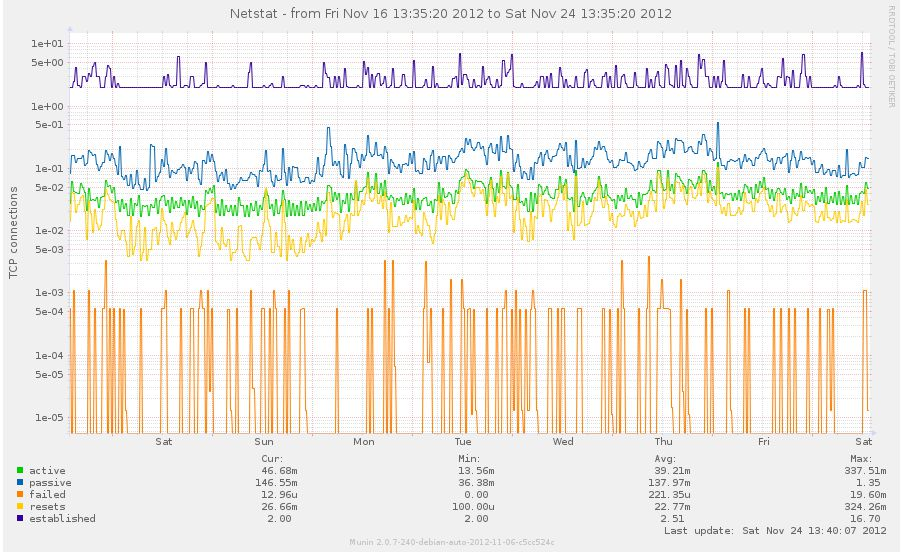
\includegraphics[width=0.8\linewidth]{munin5.png} 
\caption{Resultados de las ejecuciones de netstat durante la última semana.} 
\label{contexto:figura} 
\end{figure}


\section{Cuestión Opcional 2}
\textbf{Instale Nagios en su sistema (el que prefiera) documentando el proceso y muestre el resultado de la monitorización de su sistema comentando qué aparece.}\\

He decidido instalar Nagios en CentOS siguiendo la siguiente guía oficial de instalación \cite{14}, en primer lugar hay que tener instalado una serie de paquetes entre ellos todos los que conforman \textit{LAMP} y algunas librerías más por lo que antes de empezar la instalación es necesario ejecutar antes el comando:
\begin{verbatim}
yum install -y wget httpd php gcc glib glibc-common gd gd-devel make net-snmp
\end{verbatim}
Ahora comenzamos la instalación de \textit{Nagios} para ello es necesario descargar \textit{Nagios Core}, además en mi caso instale también \textit{Nagios Plugins}. Ambos pueden obtenerse de la referencia oficial del mismo \cite{15}.
Estos pasos permiten la instalación de Nagios en centOS:
\begin{enumerate}
\item \textbf{Añadir un usuario u un grupo para \textit{Nagios}:} Nagios usa un propio usuario para la instalación y posterior configuración del mismo para ello tendremos que ejecutar los comandos:
\begin{verbatim}
useradd nagios
groupadd nagcmd
usermod -a -G nagcmd nagios
\end{verbatim}
\item \textbf{Configuración:} Cuando se descarga Nagios de la red se trata de su código fuente por lo que será necesaria una compilación después de la configuración necesaria, después de descomprimir el archivo usamos el comando cd para situarnos en el directorio que contiene los archivos de \textit{Nagios Core} y ejecutamos en primer lugar:
\begin{verbatim}
./configure --with-nagios-group=nagcmd
\end{verbatim}
En mi caso se produjo un error, al escribir el grupo de usuarios no se realizó de forma correcta y por tanto la configuración no se realizó satisfactoriamente, pero no muestra señales de error hasta que no se avanza en la instalación.
\item \textbf{Compilación e instalación:} Una vez configurado pasamos a compilarlo con el comando \textit{make} ahora instalamos Nagios junto con una serie de módulos con los comandos:
\begin{verbatim}
make install
make install-init
make install-config
make install-commandmode
make install-webconf
\end{verbatim}
Con esto instalamos todas las configuraciones, en mi caso me di cuenta del error anterior cuando ejecute \textit{make install-commandmode} que obtenía un error de salida. Por último concluimos la instalación con los siguientes comandos:
\begin{verbatim}
cp -R contrib/eventhandlers/ /usr/local/nagios/libexec/
chown -R nagios:nagios /usr/local/nagios/libexec/eventhandlers
/usr/local/nagios/bin/nagios -v /usr/local/nagios/etc/nagios.cfg
\end{verbatim}
Por último iniciamos el servicio de Nagios:
\begin{verbatim}
/etc/init.d/nagios start
\end{verbatim}
\item \textbf{Establecer el password del usuario por defecto:} Haciendo uso de la orden:
\begin{verbatim}
htpasswd –c /usr/local/nagios/etc/htpasswd.users nagiosadmin
\end{verbatim}
\item \textbf{Instalación de plugins:} De manera similar a lo anterior siguiendo los comandos:
\begin{verbatim}
cd /tmp/nagios-plugins-2.0
./configure --with-nagios-user=nagios --with-nagios-group=nagios
make
make install
\end{verbatim}
\end{enumerate}
Para acceder al monitor tenemos que hacerlo a través de su interfaz web a través de la dirección \textit{http://<IP>/nagios} en nuestro caso \textit{http://localhost/nagios} (figura 32).\\
Con él podremos comprobar la información del servidor en todo momento, desde otra terminal, nos aporta mucha información del sistema, tiene una página que lista los hosts que se encuentran en linea (figura 33) y los servicios de este (figura 34). Ahora está todo correcto pero en caso de que se produzcan incidencias el se indica en la parte superior del mismo dependiendo del host como el que aparece en la figura 33, además también se puede comprobar la información de cada uno de los servicios en todo momento y modificar los chequeos sobre el mismo, y las notificaciones en el sistema.
\begin{figure}[H]
\centering 
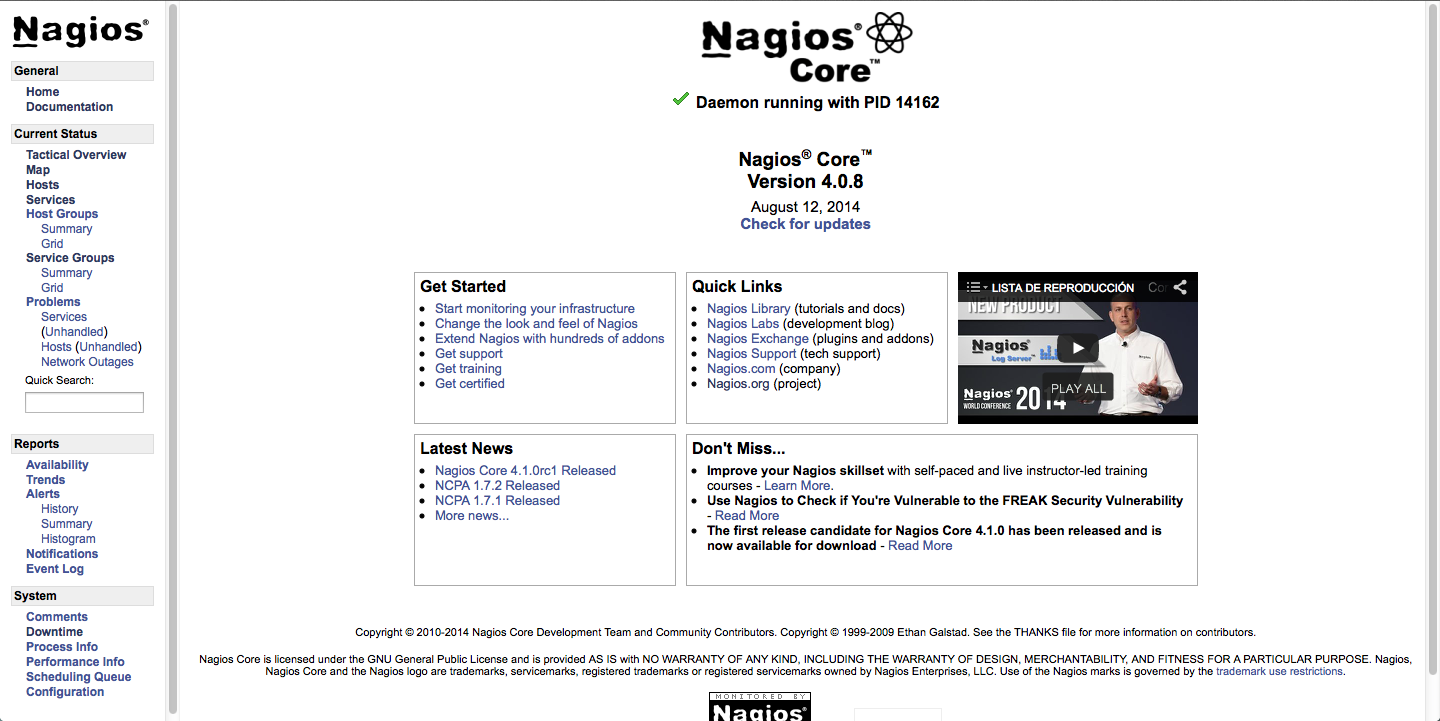
\includegraphics[width=1\linewidth]{nagios1.png} 
\caption{Nagios instalado funcionando en centOS.} 
\label{contexto:figura} 
\end{figure}
 \begin{figure}[H]
\centering 
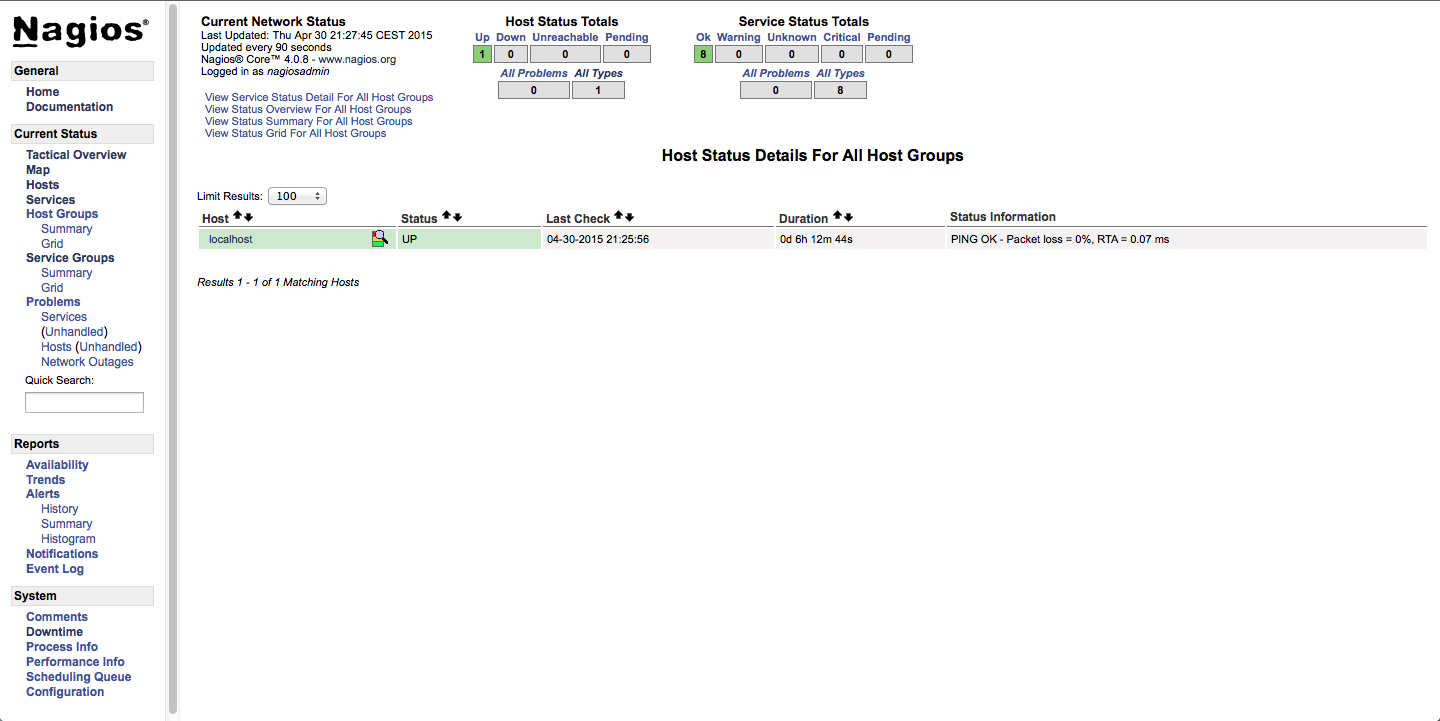
\includegraphics[width=1\linewidth]{nagios2.png} 
\caption{Estado de todos los hosts.} 
\label{contexto:figura} 
\end{figure}
\begin{figure}[H]
\centering 
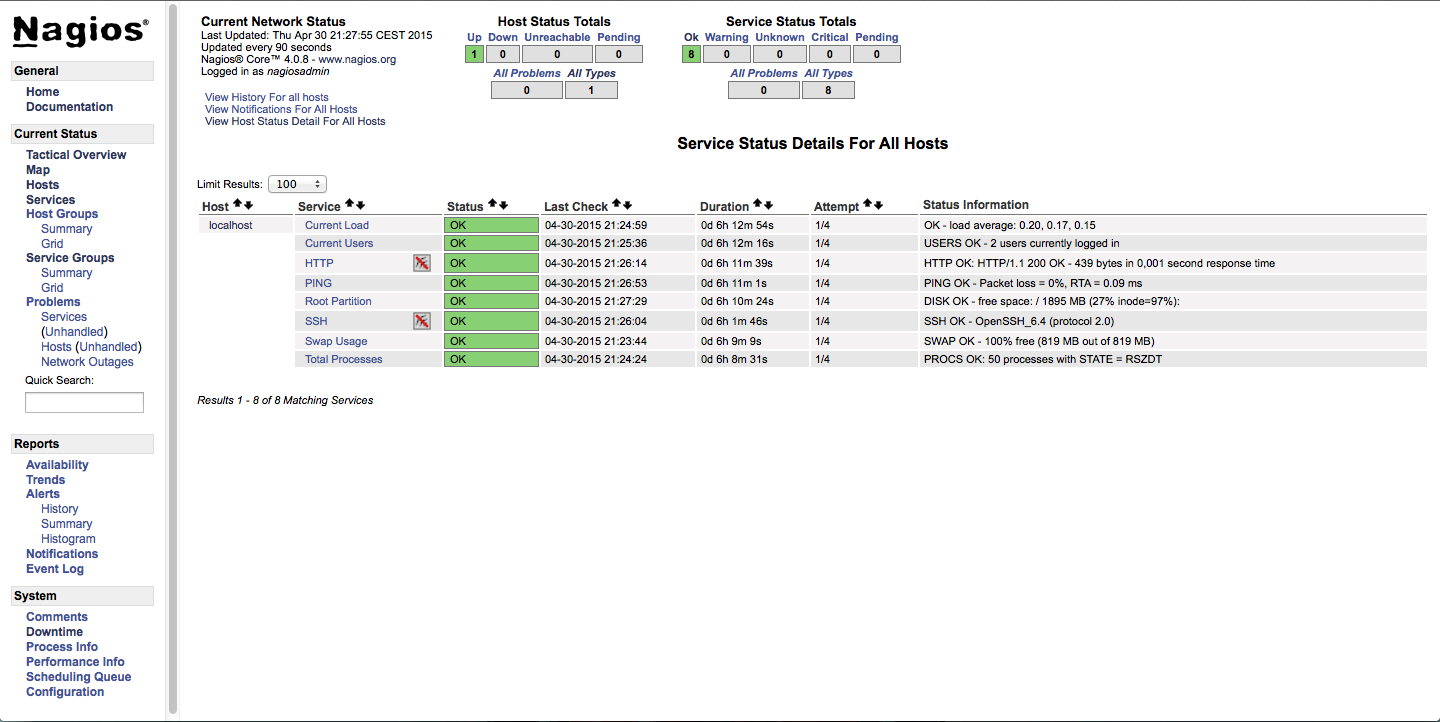
\includegraphics[width=1\linewidth]{nagios3.png} 
\caption{Estados de los servicios del host.} 
\label{contexto:figura} 
\end{figure}
\begin{figure}[H]
\centering 
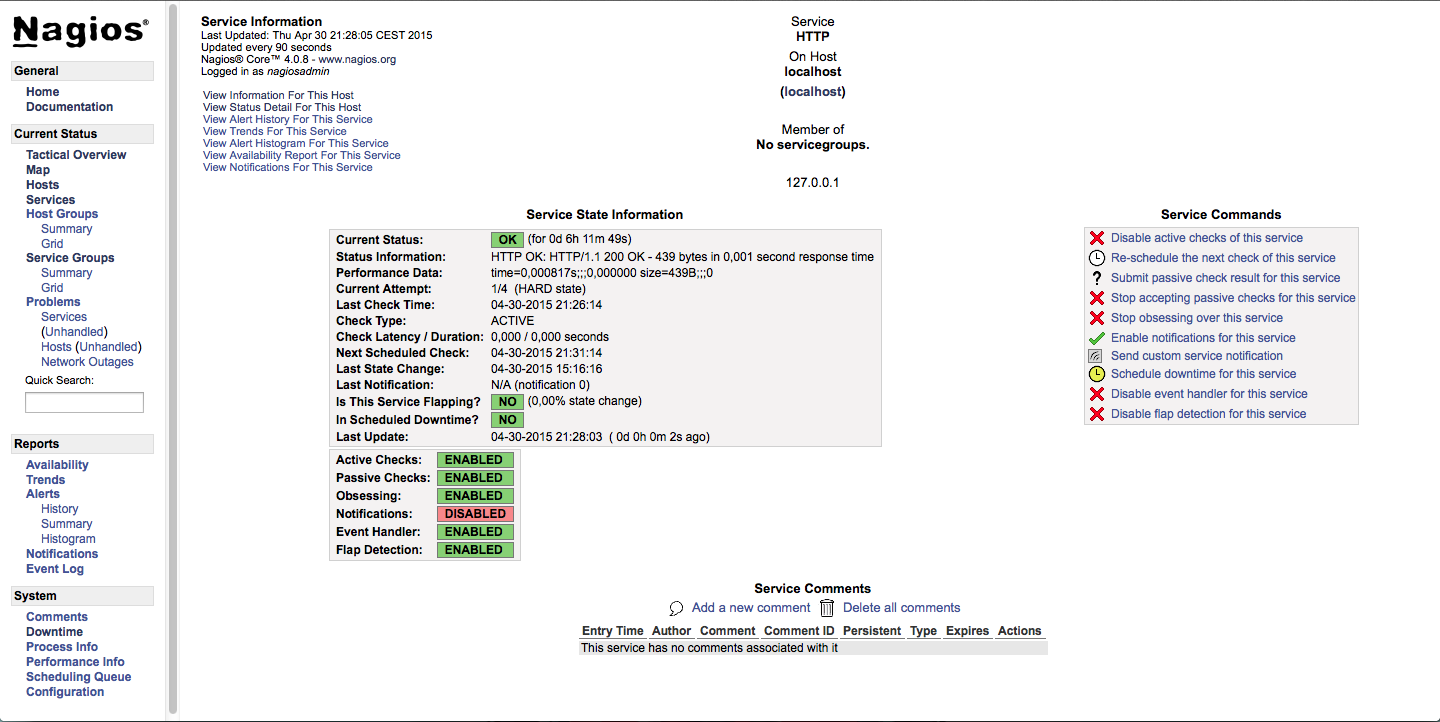
\includegraphics[width=1\linewidth]{nagios4.png} 
\caption{Estado del servicio HTTP.} 
\label{contexto:figura} 
\end{figure}
\textit{Nagios} es un monitor que da muchas posibilidades debido a que se pueden agregar plugins para ampliar su funcionamiento, por ejemplo en mi caso queremos obtener información de la carga de \textit{CPU}, \textit{Nagios} por defecto no tiene un plugin que muestra esta información de forma directa e interpretable por lo que he optado por la instalación de un plugin llamado \textit{pnp4nagios} que da información de los host y servicios del sistema. El proceso de instalación es similar, descargamos \textit{pnp4nagios} de la referencia oficial \cite{16}, descomprimimos el archivo y ejecutamos:
\begin{verbatim}
./configure
make all
make install
make install-webconf
make install-config
make install-init
\end{verbatim}
Ahora procedemos a su configuración, en primer lugar nos dirigimos a \textit{/usr/local/nagios/etc/nagios.cfg} y añadimos una serie de lineas:
\begin{verbatim}

process_performance_data=1

host_perfdata_file=/usr/local/pnp4nagios/var/host-perfdata
service_perfdata_file=/usr/local/pnp4nagios/var/service-perfdata

host_perfdata_file_template=DATATYPE::HOSTPERFDATA\tTIMET::$TIMET$\tHOSTNAME::
$HOSTNAME$\tHOSTPERFDATA::$HOSTPERFDATA$\tHOSTCHECKCOMMAND::$HOSTCHECKCOMMAND$\tHOSTSTATE::
$HOSTSTATE$\tHOSTSTATETYPE::$HOSTSTATETYPE$\tHOSTOUTPUT::$HOSTOUTPUT$
service_perfdata_file_template=DATATYPE::SERVICEPERFDATA\tTIMET::$TIMET$\tHOSTNAME::
$HOSTNAME$\tSERVICEDESC::$SERVICEDESC$\
tSERVICEPERFDATA::$SERVICEPERFDATA$\tSERVICECHECKCOMMAND::$SERVICECHECKCOMMAND$\tHOSTSTATE::
$HOSTSTATE$\tHOSTSTATETYPE::
$HOSTSTATETYPE$\tSERVICESTATE::$SERVICESTATE$\
tSERVICESTATETYPE::$SERVICESTATETYPE$\tSERVICEOUTPUT::$SERVICEOUTPUT$

host_perfdata_file_mode=a
service_perfdata_file_mode=a

host_perfdata_file_processing_interval=15
service_perfdata_file_processing_interval=15

host_perfdata_file_processing_command=process-host-perfdata-file
service_perfdata_file_processing_command=process-service-perfdata-file
\end{verbatim}
(El texto a añadir está simplificado para una uso correcto dirijase a la referencia \cite{17}). Esta es la configuración que va a permitir a pnp4nagios adherirse a Nagios y comenzar a realizar los registros de datos (figura 36). Ahora nos dirigimos al archivo \textit{/usr/local/nagios/etc/templates.cfg} para añadir dos templates, esto nos servirá para que la interfaz web de Nagios entienda que existe información de los servicios y los host y que debe mostrarse:
\begin{verbatim}
define host {
name            host-pnp
action_url      /pnp4nagios/index.php/graph?host=$HOSTNAME$&srv=_HOST_
register        0
}

define service {
name            srv-pnp
action_url      /pnp4nagios/index.php/graph?host=$HOSTNAME$&srv=$SERVICEDESC$
register        0
}
\end{verbatim}
Por último nos dirigimos al archivo \textit{/usr/local/nagios/etc/localhost.cfg} para terminar la configuración, y ya tan solo tenemos que agregar los templates creados a los servicios y hosts declarados en este archivo, en mi caso lo hice con el servicio PING (figura 39) y la máquina local (figuras 37, 38, 40). Podemos comprobar que \textit{pnp4nagios} funciona accediendo a la dirección \textit{http://localhost/pnp4nagios}, un fallo posterior a la instalación que impedía que se mostrasen los datos proporcionados por el plugin fue que el plugin hace uso de Apache y después de la instalación para que esta funcione correctamente es necesario reiniciar el servicio de Nagios y apache para ello se usa:
\begin{verbatim}
service httpd restart
service nagios restart
\end{verbatim}
Después de esto ya tendremos \textit{pnp4nagios} operativo.
\begin{figure}[H]
\centering 
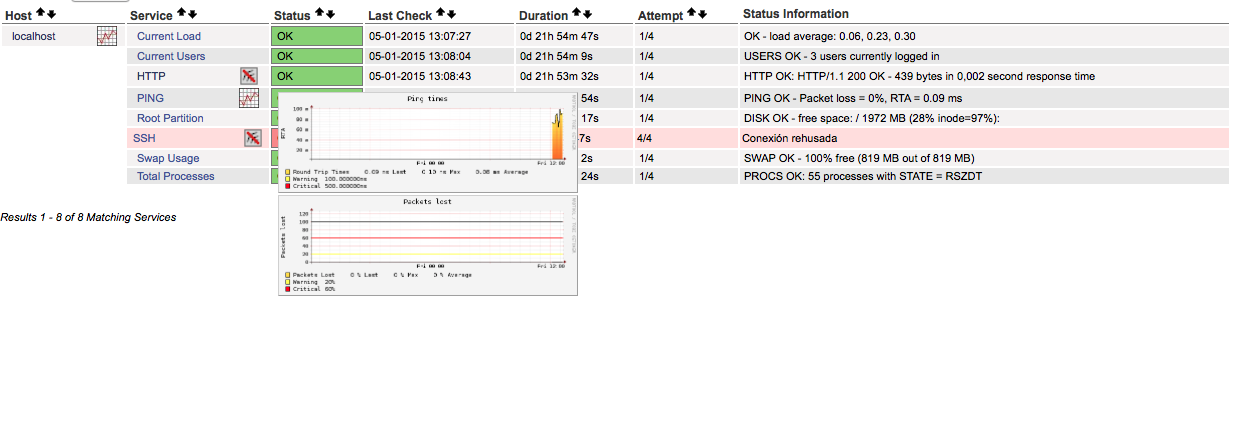
\includegraphics[width=1\linewidth]{nagios5.png} 
\caption{Nagios configurado para que muestre información de pnp4nagios.} 
\label{contexto:figura} 
\end{figure}
\begin{figure}[H]
\centering 
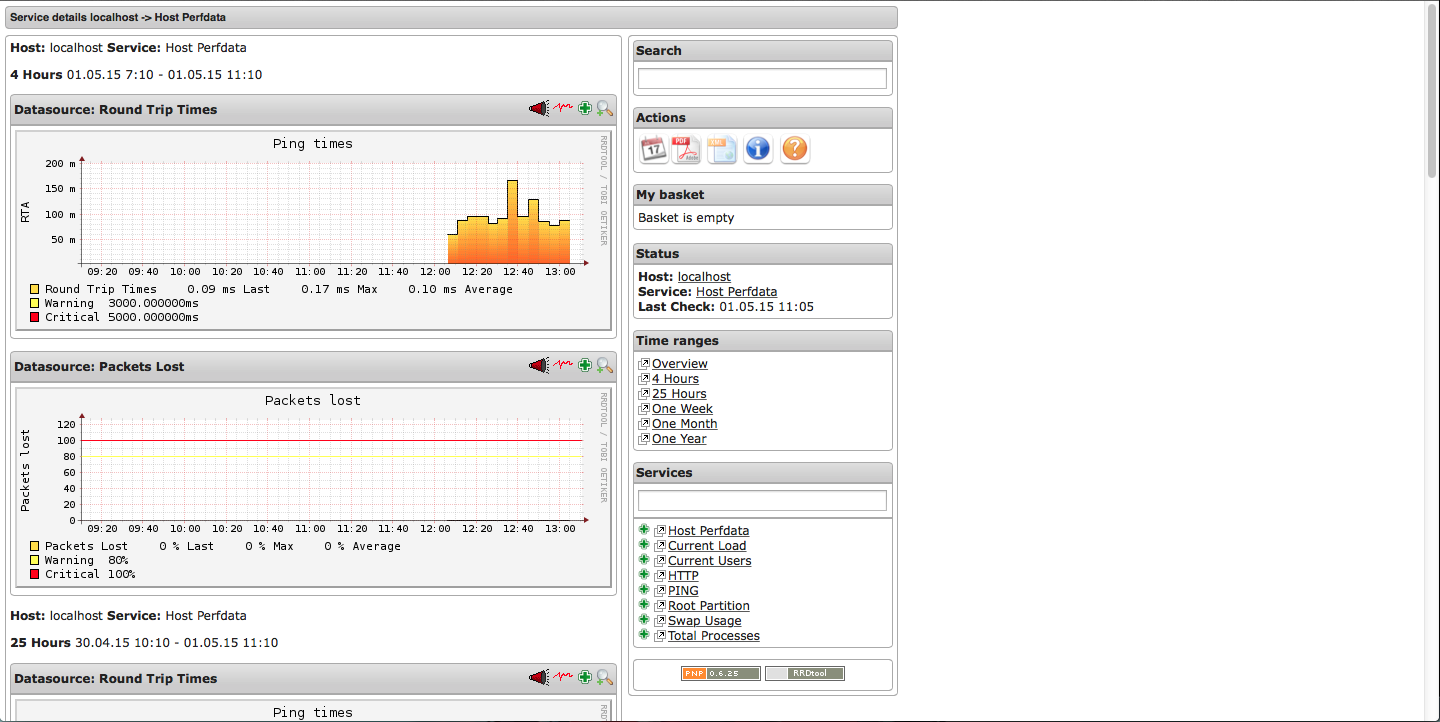
\includegraphics[width=1\linewidth]{nagios6.png} 
\caption{Estado del host, paquetes perdidos.} 
\label{contexto:figura} 
\end{figure}
\begin{figure}[H]
\centering 
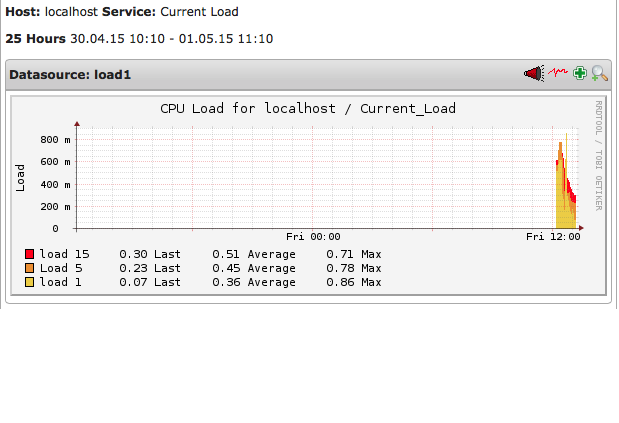
\includegraphics[width=1\linewidth]{nagios7.png} 
\caption{Carga del sistema del Host.} 
\label{contexto:figura} 
\end{figure}
\begin{figure}[H]
\centering 
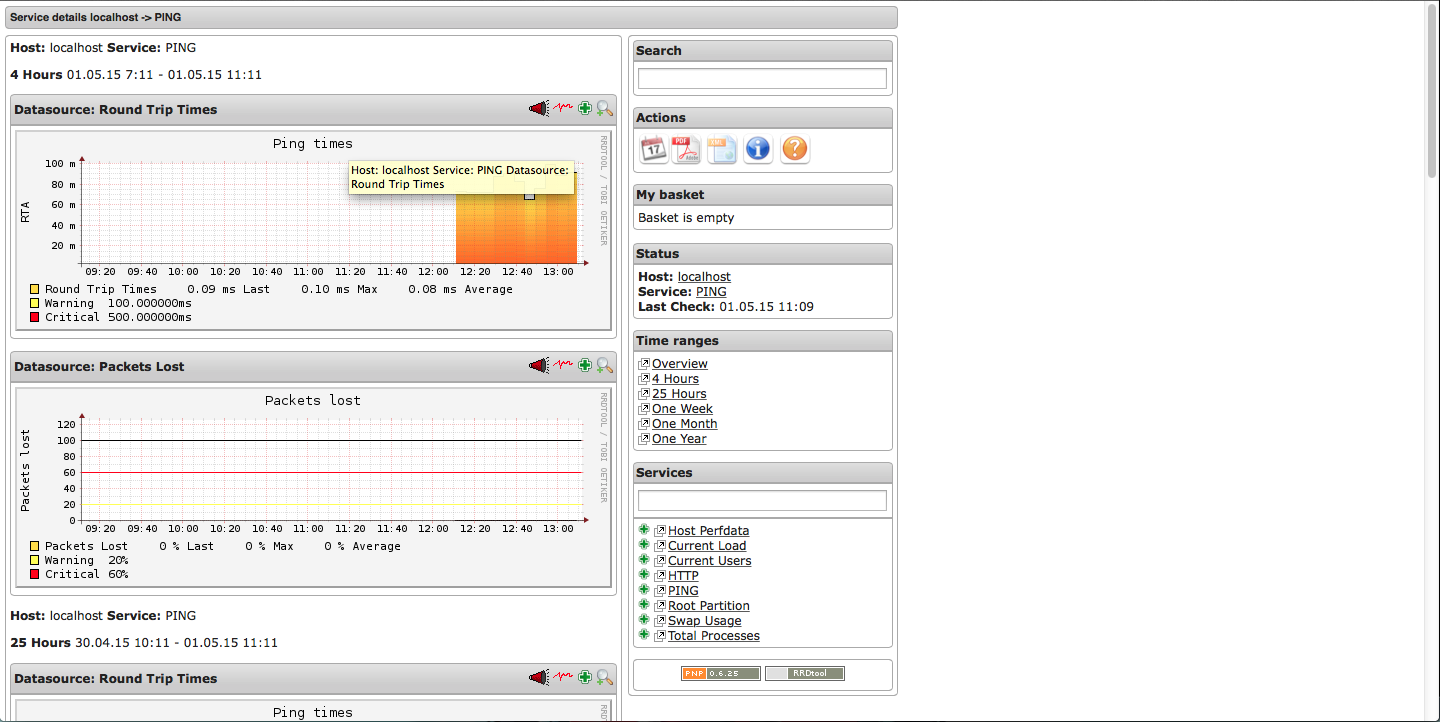
\includegraphics[width=1\linewidth]{nagios8.png} 
\caption{Estado del servicio PING.} 
\label{contexto:figura} 
\end{figure}
\begin{figure}[H]
\centering 
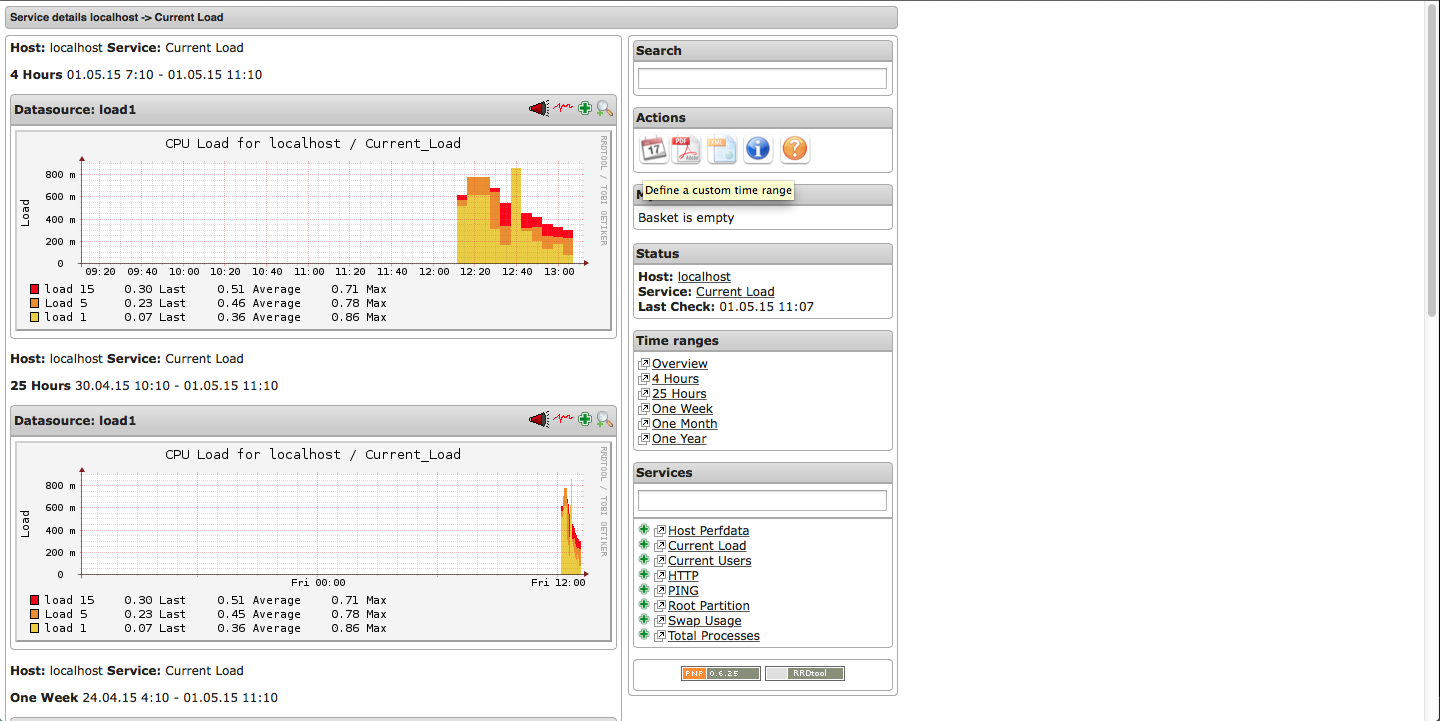
\includegraphics[width=1\linewidth]{nagios9.png} 
\caption{Información extensa sobre la carga del sistema.} 
\label{contexto:figura} 
\end{figure}

\section{Cuestión 8}
\textbf{Escriba un breve resumen sobre alguno de los artículos donde se muestra el uso de strace o busque otro y coméntelo.}\\

Tras haber leído el artículo \url{http://blog.softlayer.com/2013/sysadmin-tips-and-tricks-using-strace-to-monitor-system-calls#utm_source=twitter&utm_medium=social&utm_content=beyond-the-command-line-with-strace&utm_campaign=blog_development-tips-and-tricks} y tomar un poco más de información de las siguientes referencias: \cite{18} \cite{19}, he llegado a la conclusión de que strace es un monitor de llamadas al sistema que puede sernos útil para comprender qué es lo que ocurre cuando un programa nos falla pero no parece ser por un fallo del programa sino del sistema, aunque se nos deja claro que no es una herramienta de debug, sino de administración de sistemas.\\
Aprendemos que usarlo es muy sencillo, simplemente se ejecuta una orden de bash: ya sea abrir un archivo, crear una carpeta, ejecutar un programa; cualquier cosa. Y strace nos mostrará la secuencia de llamadas al sistema que se han realizado para realizar la acción indicada.\\
El artículo en cuestión nos muestra y expande una serie de ejemplos concretos, lo cual nos ayuda a comprender strace mejor, pero en lugar de comentar dichos ejemplos, será más útil si muestro un ejemplo y lo comento yo mismo.\\
Probemos strace para un programa en c, por ejemplo el clásico hello world, veamos qué hace strace:
\begin{figure}[H]
\centering 
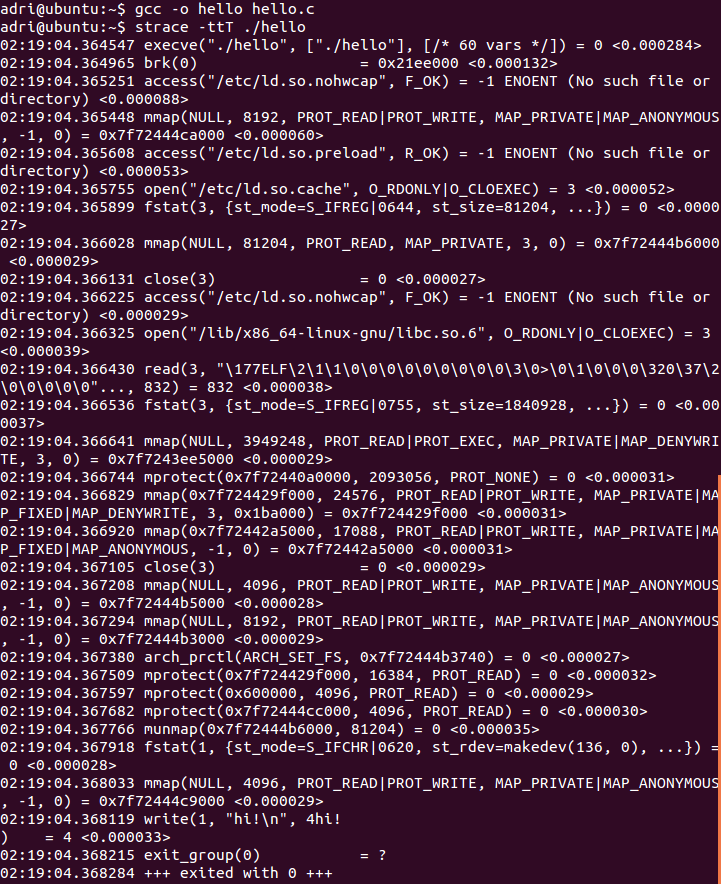
\includegraphics[width=0.8\linewidth]{strace.png} 
\caption{Ejecución de strace para el hello world de C.} 
\label{contexto:figura} 
\end{figure}

Como podemos ver, la ejecución de un archivo es muy compleja a nivel de sistema, incluso para un programa tan sencillo como el hello world, veamos algunos detalles que pueden ser interesantes:\\
Cuando el programa se ejecuta, el binario se le pasa a \textit{execv}, el heap se extiende con una llamada a \textit{brk} y algunas regiones de RAM se mapean para las librerias compartidas. Por último podemos ver que se llama a write con un descriptor de archivo 1, nuestro mensaje, y la longitud. Este strace nos hace ver el coste de iniciar cualquier ejecutable, y las llamadas al sistema que se producen en dicha ejecución.

\pagebreak

\section{Cuestión 9}
\textbf{Acceda a la consola mysql (o a través de phpMyAdmin) y muestre el resultado de mostrar el ”profile” de una consulta (la creación de la BD y la consulta la puede hacer líbremente).}\\

\cite{20} \cite{21} La BD implementada tiene 4 tablas llamadas proveedor, pieza, proyecto y ventas, se trata de un problema en el que cada venta consta de una pieza por parte de un proveedor destinado para un proyecto. El código sql que vamos a usar para generar las tablas es el siguiente:

\begin{verbatim}
CREATE TABLE proveedor(
codpro char(3) not null,
nompro varchar(30) not null,
status int,
ciudad varchar(15),
primary key (codpro) );

CREATE TABLE pieza(
codpie char(3) not null,
nompie varchar(10) not null,
color  varchar(10),
peso   decimal(4),
ciudad varchar(15),
primary key (codpie) );

CREATE TABLE proyecto(
codpj  char(3) not null,
nompj  varchar(20) not null,
ciudad varchar(15),
primary key (codpj) );

CREATE TABLE ventas(
codpro char(3) references proveedor(codpro),
codpie char(3) references pieza(codpie),
codpj  char(3) references proyecto(codpj),
cantidad decimal(4),
primary key (codpro,codpie,codpj) );
\end{verbatim}

\pagebreak

Para iniciar el profiler de mysql tenemos que ejecutar la sentencia siguiente:
\begin{figure}[H]
\centering 
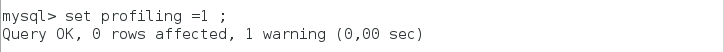
\includegraphics[width=1\linewidth]{BD1.png} 
\caption{Activando el profiler.} 
\label{contexto:figura} 
\end{figure}

Ya que por defecto está establecido a 0 y no hace uso del profiler. Ahora debemos seleccionar la base de datos que vamos a usar para ello se creó una BD llamada \textit{Practica}:
\begin{figure}[H]
\centering 
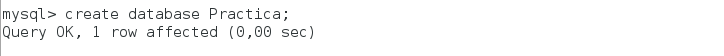
\includegraphics[width=1\linewidth]{BD2.png} 
\caption{Creación de la BD Practicas.} 
\label{contexto:figura} 
\end{figure}

\begin{figure}[H]
\centering 
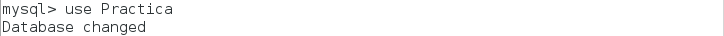
\includegraphics[width=1\linewidth]{BD3.png} 
\caption{Selección base de datos Practicas.} 
\label{contexto:figura} 
\end{figure}

Ejecutamos las sentencias de creación de tablas anteriormente mostrado con el siguiente comando, ya que están almacenadas en un archivo llamado tablas.sql:
\begin{figure}[H]
\centering 
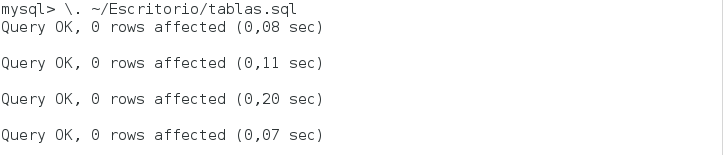
\includegraphics[width=1\linewidth]{BD4.png} 
\caption{Creacion de las tablas.} 
\label{contexto:figura} 
\end{figure}

\pagebreak

Ahora que hemos creado las tablas vamos a ver que ha ocurrido en el profiler:
\begin{figure}[H]
\centering 
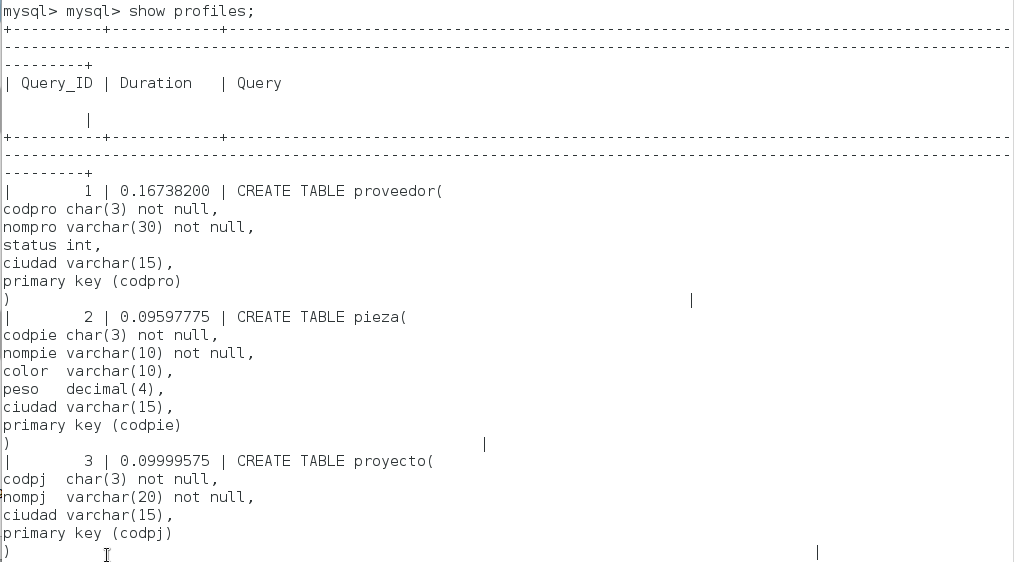
\includegraphics[width=1\linewidth]{BD5.png} 
\caption{Estado profiler despues de crear tablas I.} 
\label{contexto:figura} 
\end{figure}

\begin{figure}[H]
\centering 
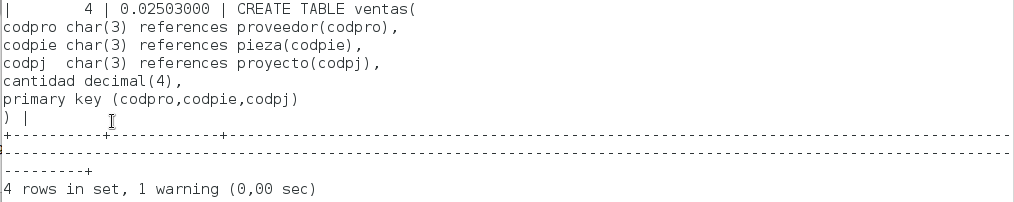
\includegraphics[width=1\linewidth]{BD6.png} 
\caption{Estado profiler despues de crear tablas II.} 
\label{contexto:figura} 
\end{figure}

Como podemos darnos cuenta el profiler da información acerca de el orden de introducción de las consultas, la duración de las mismas y cuál fue la consulta, esto lo podemos conocer con el comando ''show profiles;'', sin embargo si queremos conocer cuanto información acerca de cuanto tardó explicitamente la consulta anterior se usa ''show profile [option]''. Para probar nuestra base de datos vamos a introducir un conjunto de valores en ella por ejemplo:

\begin{verbatim}
INSERT INTO proveedor VALUES ('S1','Jose', 2, 'Madrid');
INSERT INTO proveedor VALUES ('S2','Manuel', 1, 'Londres');
INSERT INTO proveedor VALUES ('S3','Luisa', 3, 'Lisboa');
INSERT INTO proveedor VALUES ('S4','Pedro', 4, 'Paris');
INSERT INTO proveedor VALUES ('S5','Maria', 5, 'Roma');


INSERT INTO pieza VALUES ('P1','Tuerca', 'Gris', 1, 'Madrid');
INSERT INTO pieza VALUES ('P2','Tornillo', 'Rojo', 1.5, 'Paris');
INSERT INTO pieza VALUES ('P3','Arandela', 'Blanco', 4, 'Lisboa');

INSERT INTO proyecto VALUES ('J1', 'proyecto 1', 'Londres');
INSERT INTO proyecto VALUES ('J2', 'proyecto 2', 'Londres');
INSERT INTO proyecto VALUES ('J3', 'proyecto 3', 'Paris');
INSERT INTO proyecto VALUES ('J4', 'proyecto 4', 'Roma');

INSERT INTO ventas VALUES ( 'S1','P1','J1',120);
INSERT INTO ventas VALUES ( 'S1','P1','J2',100);
INSERT INTO ventas VALUES ( 'S3','P2','J3',220);
INSERT INTO ventas VALUES ( 'S5','P3','J1',300);
\end{verbatim}

Como podemos ver se puede ver cuanto ha tardado cada una de esas consultas:
\begin{figure}[H]
\centering 
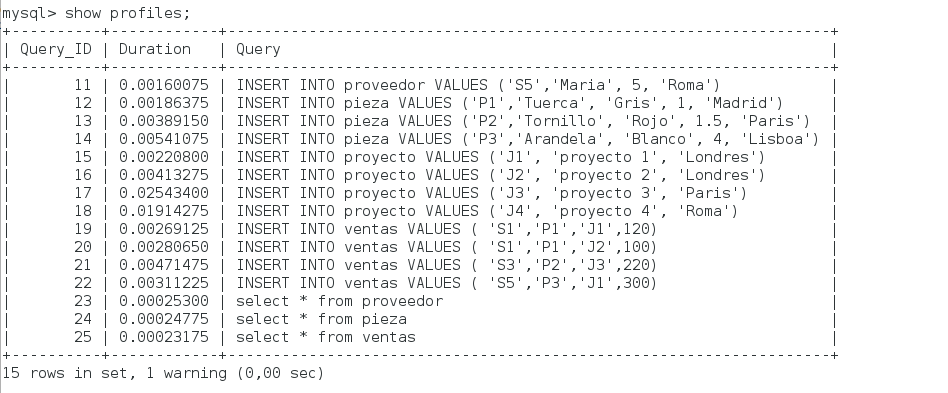
\includegraphics[width=1\linewidth]{BD7.png} 
\caption{Estado profiler despues de insertar en las tablas.} 
\label{contexto:figura} 
\end{figure}

Ahora vamos a proceder a comparar una serie de consultas utilizando el profiler:
\begin{itemize}
\item \textbf{Creación y alteración de tablas:} Normalmente una alteración de una tabla, es más costosa que una creación, esto es debido a que la alteración tiene que recrear la tabla, como podemos ver en las figuras 49-50, la creación de tablas en primer lugar tiene que ejecutar menos procesos y el más costoso de ellos es crear la propia tabla sin ambargo la alteración además de tener que completar dicho proceso de creación tiene que añadir la nueva información que se le ha dado por ello que la alteración es más costosa como podemos comprobar en la figura 51 en las entradas 26 y 27.

\begin{figure}[H]
\centering 
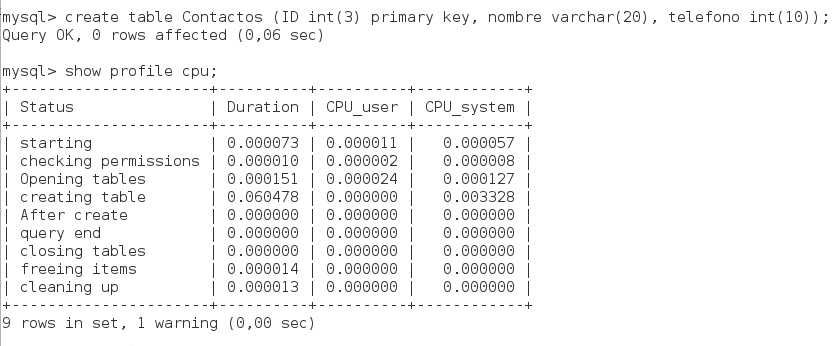
\includegraphics[width=1\linewidth]{BD8.png} 
\caption{Tiempos de creación de una tabla.} 
\label{contexto:figura} 
\end{figure}

\begin{figure}[H]
\centering 
\includegraphics[width=1\linewidth]{BD9.png} 
\caption{Tiempos de alteración de una tabla.} 
\label{contexto:figura} 
\end{figure}

\begin{figure}[H]
\centering 
\includegraphics[width=1\linewidth]{BD10.png} 
\caption{Tiempo total de creación y alteración de una tabla.} 
\label{contexto:figura} 
\end{figure}

\item \textbf{Comparación de consultas con distintas construcciones:} Se han preparado dos consultas sobre la base de datos con el mismo resultado pero con construncciones distintas, la primera de ellas (figura 52) usa un operador \textit{join}, mientras que la segunda no usa ningún operador (figura 54) como podemos comprobar el resultado es el mismo pero fijandonos en los tiempos aportados por el profiler (figuras 53-55) la consulta que usa el operador join hace mucho más uso de la CPU que la que no lo usa aunque la duración sea practicamente la misma (figura 56), no es una gran carga para la CPU sin embargo conviene cargarla lo menos posible y hacer uso de consultas optimas para ello.

\pagebreak

\begin{figure}[H]
\centering 
\includegraphics[width=1\linewidth]{BD11.png} 
\caption{Consulta I.} 
\label{contexto:figura} 
\end{figure}

\begin{figure}[H]
\centering 
\includegraphics[width=1\linewidth]{BD12.png} 
\caption{Tiempos de la consulta I.} 
\label{contexto:figura} 
\end{figure}

\pagebreak

\begin{figure}[H]
\centering 
\includegraphics[width=1\linewidth]{BD13.png} 
\caption{Consulta II.} 
\label{contexto:figura} 
\end{figure}

\begin{figure}[H]
\centering 
\includegraphics[width=1\linewidth]{BD14.png} 
\caption{Tiempos de la consulta II.} 
\label{contexto:figura} 
\end{figure}

\begin{figure}[H]
\centering 
\includegraphics[width=1\linewidth]{BD15.png} 
\caption{Tiempo total de las consultas.} 
\label{contexto:figura} 
\end{figure}
\end{itemize}

\pagebreak

\begin{thebibliography}{99}
\bibitem{1} \url{http://askubuntu.com/questions/425809/where-are-the-logs-for-apt-get}
\bibitem{2} \url{http://superuser.com/questions/147857/how-to-view-history-of-yum-commands-update-install-remove}
\bibitem{3} \url{http://manpages.ubuntu.com/manpages/jaunty/man8/logrotate.8.html}
\bibitem{4} \url{http://www.estrellateyarde.org/logs-en-linux}
\bibitem{5} \url{http://linux.die.net/man/8/mdadm}
\bibitem{6} \url{https://www.howtoforge.com/replacing_hard_disks_in_a_raid1_array}
\bibitem{7} \url{http://systemadmin.es/2011/02/anadir-o-quitar-discos-en-fallo-de-un-raid-por-software}
\bibitem{8} \url{http://es.slideshare.net/josefabiandiazs/programar-tareas-crontab-en-ubuntu}
\bibitem{9} \url{http://en.wikipedia.org/wiki/Dmesg}
\bibitem{10} \url{https://technet.microsoft.com/en-us/magazine/2008.08.pulse.aspx}
\bibitem{11} \url{https://technet.microsoft.com/en-us/library/cc722148.aspx}
\bibitem{12} \url{https://tuxpepino.wordpress.com/2007/04/27/instalar-y-configurar-lm-sensors/}
\bibitem{13} \url{http://demo.munin-monitoring.org/munin-monitoring.org/demo.munin-monitoring.org/index.html#apache}
\bibitem{14} \url{http://assets.nagios.com/downloads/nagioscore/docs/Installing_Nagios_Core_From_Source.pdf}
\bibitem{15} \url{http://www.nagios.org/download}
\bibitem{16} \url{https://docs.pnp4nagios.org}
\bibitem{17} \url{http://bitflip.net/graphing-nagios-services-with-pnp4nagios-0-6-41/}
\bibitem{18} \url{http://www.oracleyyo.com/index.php/2009/12/10/strace-comando-para-hacer-debug-a-bajo-n}
\bibitem{19} \url{http://stackoverflow.com/questions/174942/how-should-strace-be-used}
\bibitem{20} \url{http://dev.mysql.com/doc/refman/5.0/en/show-profile.html}
\bibitem{21} \url{http://www.ehu.eus/ehusfera/davidfernandez/2009/12/03/mysql-query-profiler/}
\end{thebibliography}
\end{document}